%%%%%%%%%%%%%%%%%%%%%%%%%%%%%%%%%%%%%%%%%%%%%%%%%%%%%%
% Author: Joris Marvezy                              %
% Date:   December 2025                              %
% Deep Learning Framework for Heston Model Calibration
%%%%%%%%%%%%%%%%%%%%%%%%%%%%%%%%%%%%%%%%%%%%%%%%%%%%%%

\documentclass{beamer}
\usepackage{hyperref}
\usepackage[T1]{fontenc}

% Packages
\usepackage{latexsym,amsmath,xcolor,multicol,booktabs,calligra}
\usepackage{graphicx,pstricks,listings,stackengine}
\usepackage{tikz}
\usepackage{algorithm}
\usepackage{algorithmic}

\author{Joris Marvezy}
\title{Deep Learning Framework for Heston Model Calibration}
\subtitle{Neural Network Surrogate Models for Accelerated Option Pricing}
\institute{TBS Education}
\date{December 2025}
\usepackage{TBS}
\usepackage{animate}  % For GIF animations

% Colors
\definecolor{deepblue}{rgb}{0,0,0.5}
\definecolor{deepred}{rgb}{0.6,0,0}
\definecolor{deepgreen}{rgb}{0,0.5,0}
\definecolor{halfgray}{gray}{0.55}
\definecolor{tbsblue}{RGB}{0,82,147}

\lstset{
    basicstyle=\ttfamily\small,
    keywordstyle=\bfseries\color{deepblue},
    emphstyle=\ttfamily\color{deepred},
    stringstyle=\color{deepgreen},
    numbers=left,
    numberstyle=\small\color{halfgray},
    rulesepcolor=\color{red!20!green!20!blue!20},
    frame=shadowbox,
}


\begin{document}

%===========================================
% TITLE SLIDE
%===========================================
\begin{frame}
    \vspace{-0.3cm}
    \titlepage
    \vspace{-0.4cm}
    \begin{center}
        
\includegraphics[keepaspectratio, height=1.0cm]{figures/logo-tbs-2019.jpg}
    \end{center}
\end{frame}

%===========================================
% TABLE OF CONTENTS
%===========================================
\begin{frame}{Outline}
    \tableofcontents[sectionstyle=show,subsectionstyle=show/shaded/hide,subsubsectionstyle=show/shaded/hide]
\end{frame}

%===========================================
% SECTION 1: INTRODUCTION
%===========================================
\section{Introduction}

\begin{frame}{Motivation}
    \begin{itemize}[<+-| alert@+>]
        \item \textbf{Heston Model:} Industry standard for stochastic volatility modeling
        \item \textbf{Problem:} Heston model needs FFT to be used and needs to be calibrated to market data. High-frequency trading and real-time risk management require fast calibration. However, traditional option pricing model calibration is computationally expensive
        \item \textbf{Research Question:} Can neural networks accelerate calibration while maintaining acceptable accuracy?
    \end{itemize}
\end{frame}

\begin{frame}{Research Objectives}
    \begin{block}<1->{Primary Objective}
        Develop a deep learning framework to accelerate Heston model calibration using neural network surrogate models.
    \end{block}

    \vspace{0.3cm}

    \onslide<2->{
    \begin{block}{Specific Goals}
        \begin{enumerate}[<+(2)-| alert@+>]
            \item Train neural networks to approximate Heston pricing function
            \item Compare calibration speed and accuracy against traditional FFT methods
            \item Evaluate performance across different volatility regimes
            \item Provide evidence-based deployment recommendations
        \end{enumerate}
    \end{block}
    }
\end{frame}

%===========================================
% SECTION 2: LITERATURE REVIEW
%===========================================
\section{Literature Review}

\subsection{From Black-Scholes to Stochastic Volatility}

\begin{frame}{The Black-Scholes Framework}
    \begin{block}{Black-Scholes-Merton Model (1973)}
        The foundational option pricing model with constant volatility $\sigma$:
        \begin{equation}
            dS_t = \mu S_t \, dt + \sigma S_t \, dW_t
        \end{equation}
    \end{block}

    \vspace{0.3cm}

    \begin{columns}
        \begin{column}{0.5\textwidth}
            \textbf{Advantages:}
            \begin{itemize}
                \item Analytical closed-form solution
                \item Fast computation
                \item Widely understood
            \end{itemize}
        \end{column}
        \begin{column}{0.5\textwidth}
            \textbf{Limitations:}
            \begin{itemize}
                \item Constant $\sigma$ assumption
                \item Cannot capture volatility smile
                \item Underprices OTM options
            \end{itemize}
        \end{column}
    \end{columns}
\end{frame}

\begin{frame}{The Volatility Smile Problem}
    \begin{block}{Empirical Evidence}
        \textbf{Rubinstein (1985):} Analysis of 2.5M CBOE quotes revealed OTM puts exhibit 2-4\% higher IV than ATM options. \textbf{Lamoureux \& Lastrapes (1993):} Documented strong IV autocorrelation with mean reversion.
    \end{block}

    \vspace{0.2cm}

    \begin{columns}
        \begin{column}{0.55\textwidth}
            \begin{figure}
                \centering
                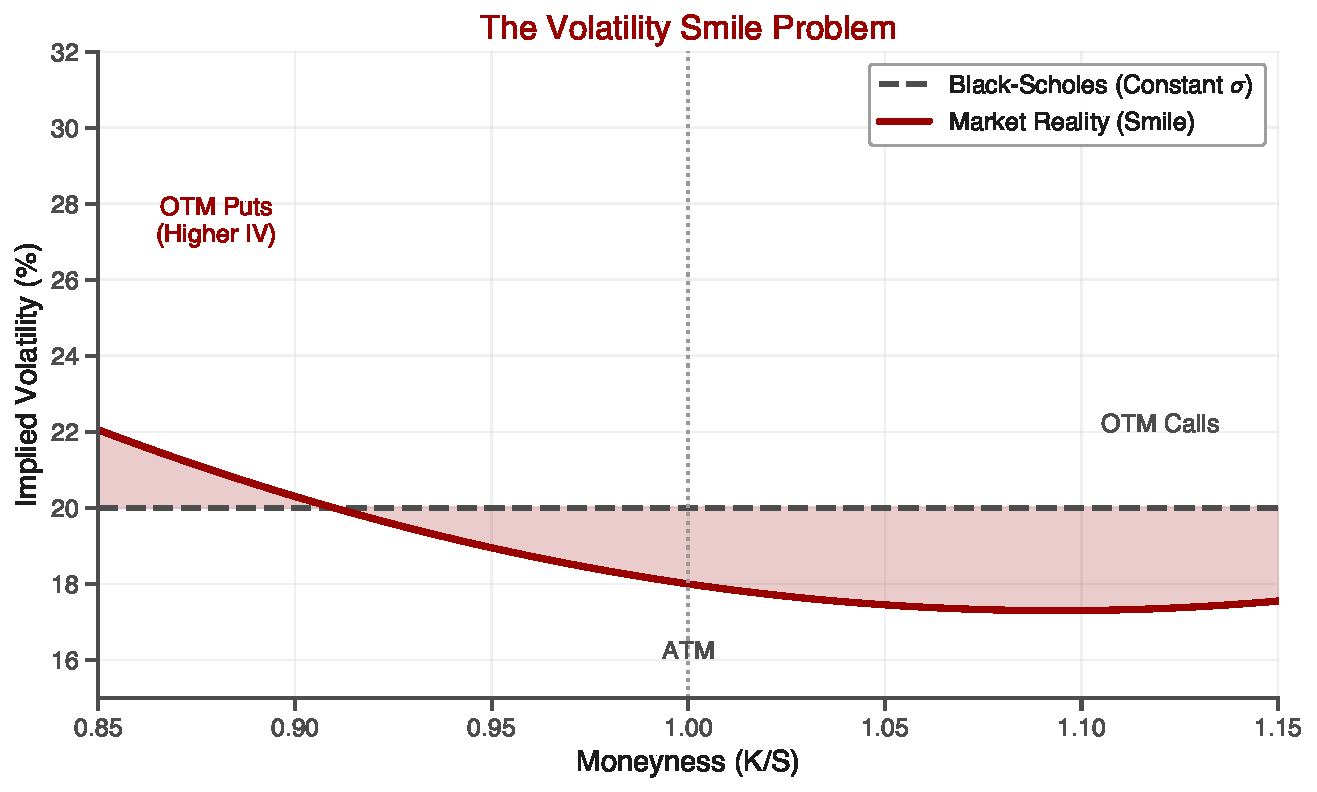
\includegraphics[width=\textwidth]{figures/volatility_smile.pdf}
            \end{figure}
        \end{column}
        \begin{column}{0.45\textwidth}
            \textbf{Key Findings:}
            \begin{itemize}
                \item OTM puts: higher IV
                \item ATM options: lower IV
                \item Post-1987: permanent skew
                \item \textbf{Black (1976):} Leverage effect ($\rho < 0$)
            \end{itemize}
        \end{column}
    \end{columns}
\end{frame}

\subsection{The Heston Stochastic Volatility Model}

\begin{frame}{The Heston Model (1993)}
    \begin{block}{Risk-Neutral Dynamics}
        Heston introduces stochastic variance with mean reversion:
        \begin{align}
            dS_t &= r S_t \, dt + \sqrt{V_t} S_t \, dW_t^S \\
            dV_t &= \kappa(\theta - V_t) \, dt + \sigma \sqrt{V_t} \, dW_t^V
        \end{align}
        where $dW_t^S \cdot dW_t^V = \rho \, dt$ captures the leverage effect.
    \end{block}

    \vspace{0.3cm}

    \begin{block}{Model Parameters}
        \begin{itemize}
            \item $v_0$: Initial variance \quad $\kappa$: Mean reversion speed
            \item $\theta$: Long-term variance \quad $\sigma$: Volatility of volatility
            \item $\rho$: Price-volatility correlation (leverage effect)
        \end{itemize}
    \end{block}
\end{frame}

\begin{frame}{Heston Model: Price Dynamics}
    \begin{figure}
        \centering
        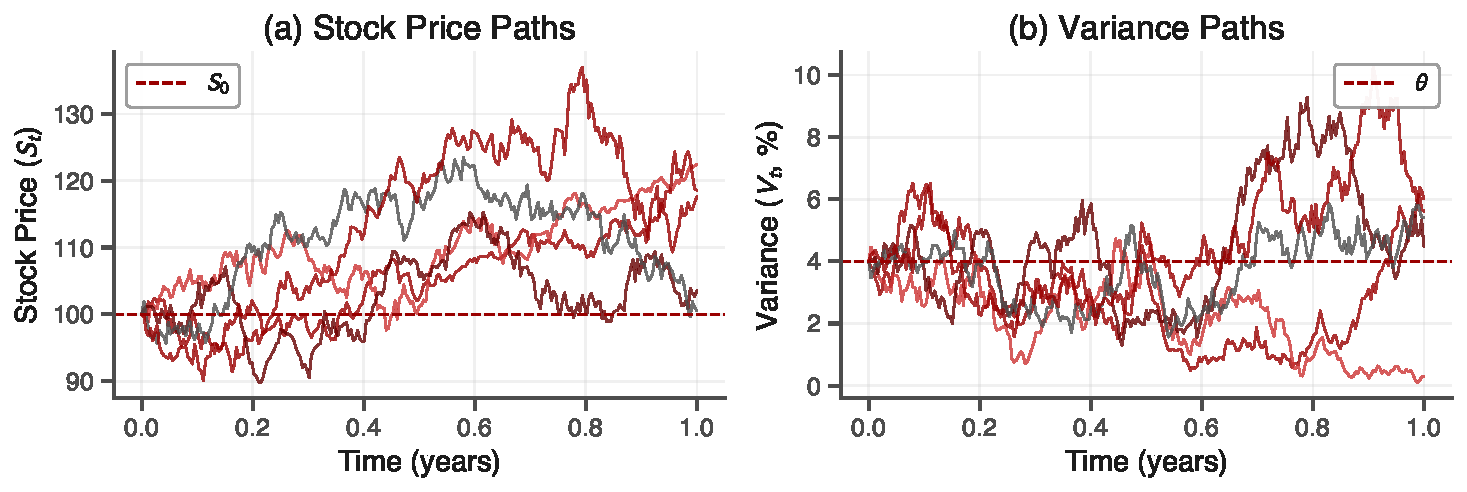
\includegraphics[width=0.95\textwidth]{figures/heston_simulation.pdf}
        \caption{Simulated Heston model paths showing mean-reverting variance}
    \end{figure}
\end{frame}

\begin{frame}{Heston Pricing via Characteristic Function}
    \begin{block}{Semi-Analytical Solution}
        Heston's key contribution: closed-form characteristic function enabling FFT pricing (Carr-Madan, 1999):
        \begin{equation}
            C(K) = \frac{e^{-\alpha \ln K}}{\pi} \int_0^\infty e^{-iv \ln K} \psi(v) \, dv
        \end{equation}
    \end{block}

    \vspace{0.3cm}

    \begin{columns}
        \begin{column}{0.5\textwidth}
            \textbf{FFT Implementation:}
            \begin{itemize}
                \item Complexity: $O(N \log N)$
                \item Grid size: $N = 4096$
                \item Damping: $\alpha = 1.5$
            \end{itemize}
        \end{column}
        \begin{column}{0.5\textwidth}
            \textbf{The Challenge:}
            \begin{itemize}
                \item Accurate but slow
                \item Milliseconds per option
                \item Calibration: 100s of calls
            \end{itemize}
        \end{column}
    \end{columns}
\end{frame}

\subsection{The Calibration Problem}

\begin{frame}{Model Calibration: The Bottleneck}
    \begin{block}{The Calibration Problem (Cont \& Tankov, 2004)}
        Finding parameters $\Theta^* = \{v_0, \kappa, \theta, \sigma, \rho\}$ minimizing pricing errors:
        \begin{equation}
            \Theta^* = \arg\min_\Theta \sum_{i=1}^N \left(C_i^{\text{market}} - C_i^{\text{model}}(\Theta)\right)^2
        \end{equation}
    \end{block}
    \footnotesize
    \textbf{Theoretical Challenges:}
    \begin{enumerate}
        \item The calibration objective typically admits \textbf{multiple local minima}, reflecting parameter non-uniqueness
        \item Some parameters, particularly \textbf{volatility-of-volatility} $\sigma$, are \textbf{poorly identified} from price data alone
        \item Different parameter combinations can produce \textbf{near-identical prices} over calibration ranges
        \item Solution stability \textbf{deteriorates with sparse or illiquid} option data
    \end{enumerate}
\end{frame}

\subsection{Neural Networks for Option Pricing}

\begin{frame}{Machine Learning Approaches}
    \begin{itemize}
        \item \textbf{Hutchinson, Lo \& Poggio (1994):} Pioneering work: neural networks can learn pricing functions without explicit model specification
        \item \textbf{Liu, Oosterlee \& Bohte (2019):} Neural networks for fast implied volatility computation
        \item \textbf{Horváth, Muguruza \& Tomas (2019):} Deep learning volatility surrogate models achieving 1000$\times$ speedup
        \item \textbf{Key Insight:} Neural networks as \textit{surrogate models}, approximating expensive pricing functions for fast inference
    \end{itemize}

    \vspace{0.3cm}

    \begin{alertblock}{Research Gap}
        Prior work lacks rigorous empirical validation on real market data across diverse volatility regimes with fair benchmarking against industrial-grade FFT methods.
    \end{alertblock}
\end{frame}

%===========================================
% SECTION 3: METHODOLOGY
%===========================================
\section{Methodology}

\subsection{Research Design}

\begin{frame}{Methodology Overview}
    \begin{figure}
        \centering
        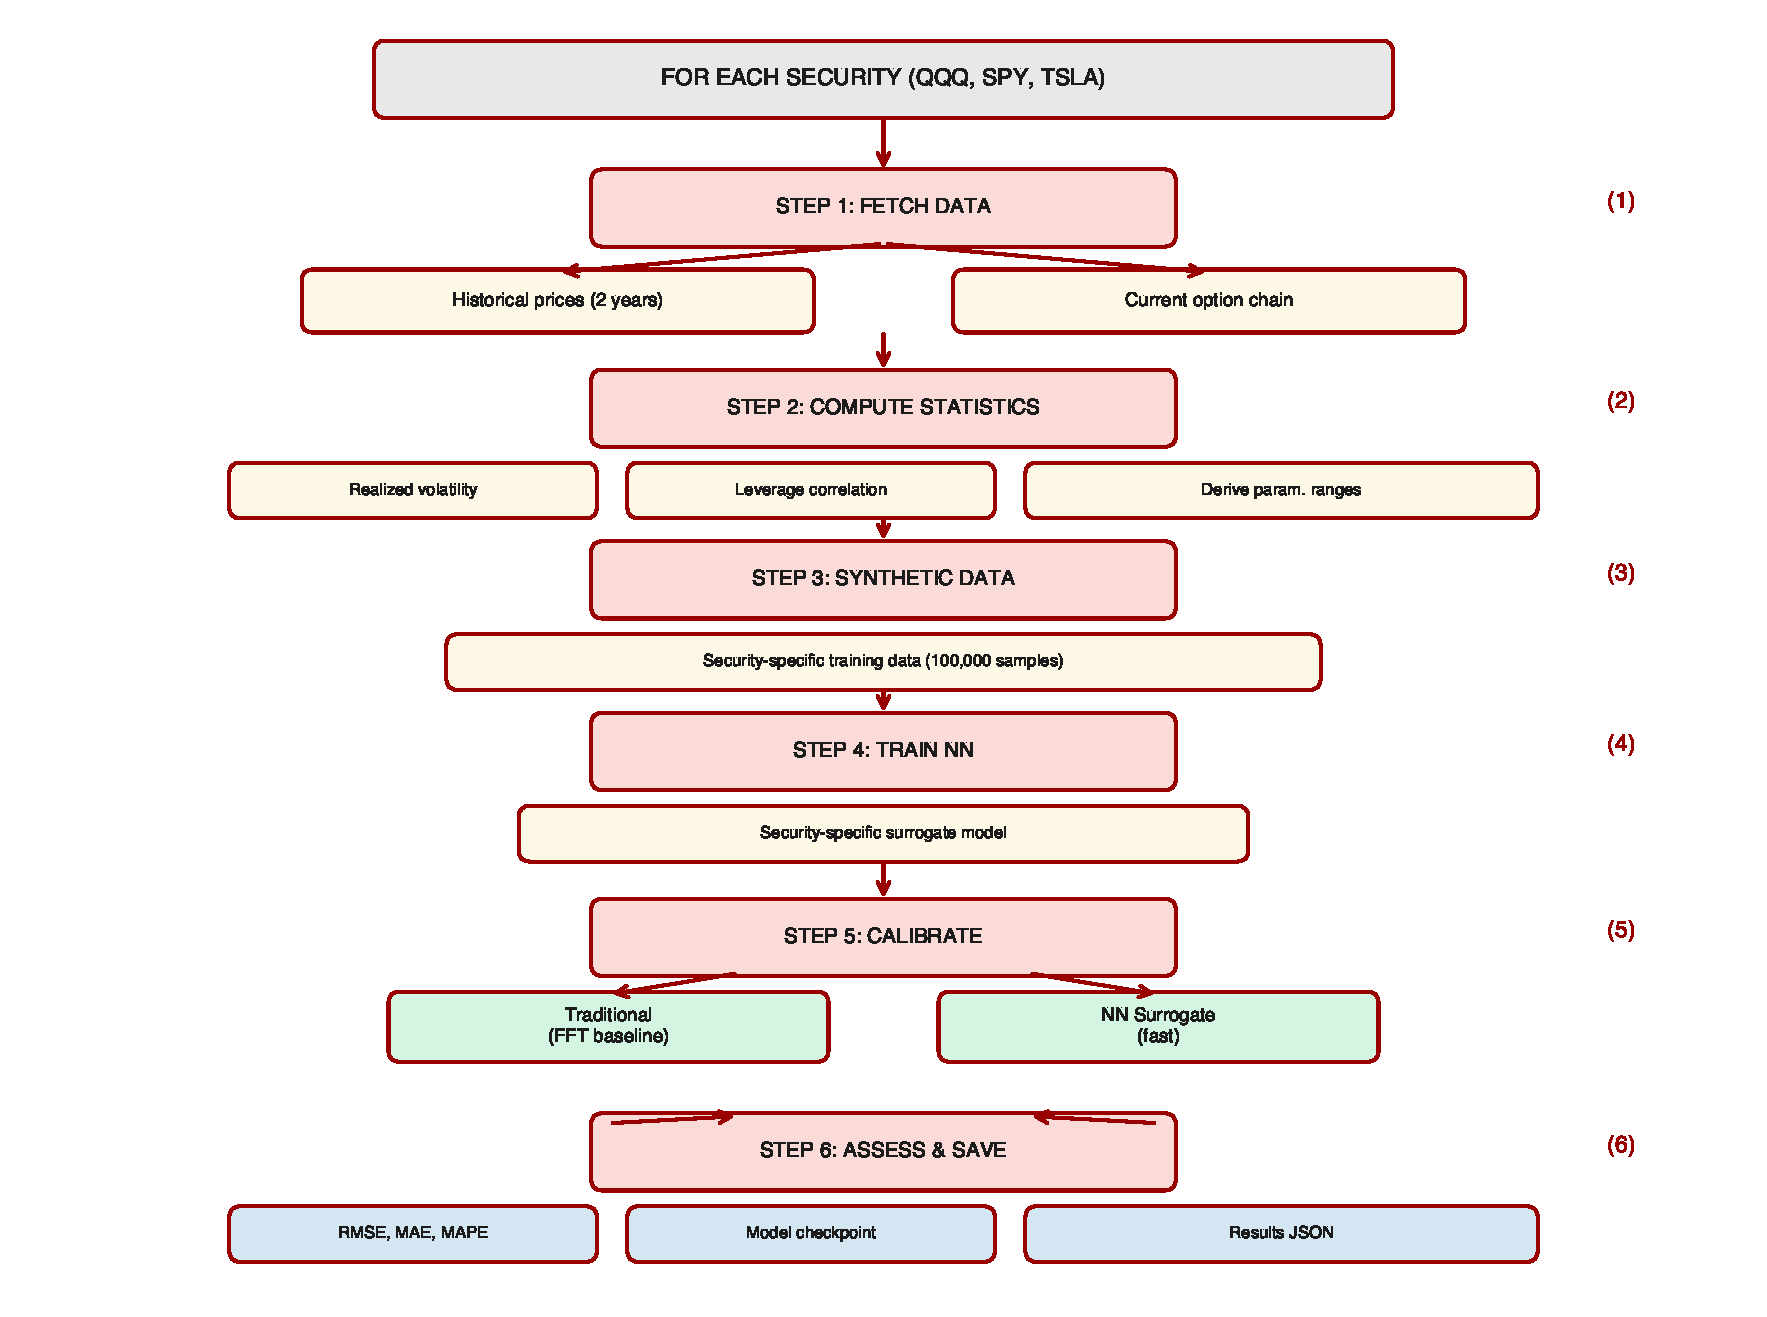
\includegraphics[width=0.85\textwidth]{figures/methodology_diagram.pdf}
        \caption{End-to-end research methodology: six-stage pipeline per security}
    \end{figure}
\end{frame}

\subsection{Data Collection}

\begin{frame}{Data Sources}
    \begin{columns}
        \begin{column}{0.5\textwidth}
            \textbf{Market Data:}
            \begin{itemize}
                \item Options: Yahoo Finance API
                \item Underlying: Historical prices
                \item Rates: US Treasury curves
            \end{itemize}
        \end{column}
        \begin{column}{0.5\textwidth}
            \textbf{Filtering Criteria:}
            \begin{itemize}
                \item Moneyness: 0.90 - 1.10
                \item Maturity: 0.05 - 1.5 years
                \item Call options, min vol: 50
            \end{itemize}
        \end{column}
    \end{columns}

    \vspace{0.5cm}

    \begin{alertblock}{Quality Assurance}
        Data filtered for liquidity and relevance, focusing on near-the-money options with sufficient trading volume.
    \end{alertblock}
\end{frame}

\begin{frame}{Data Collection Pipeline}
    \begin{figure}
        \centering
        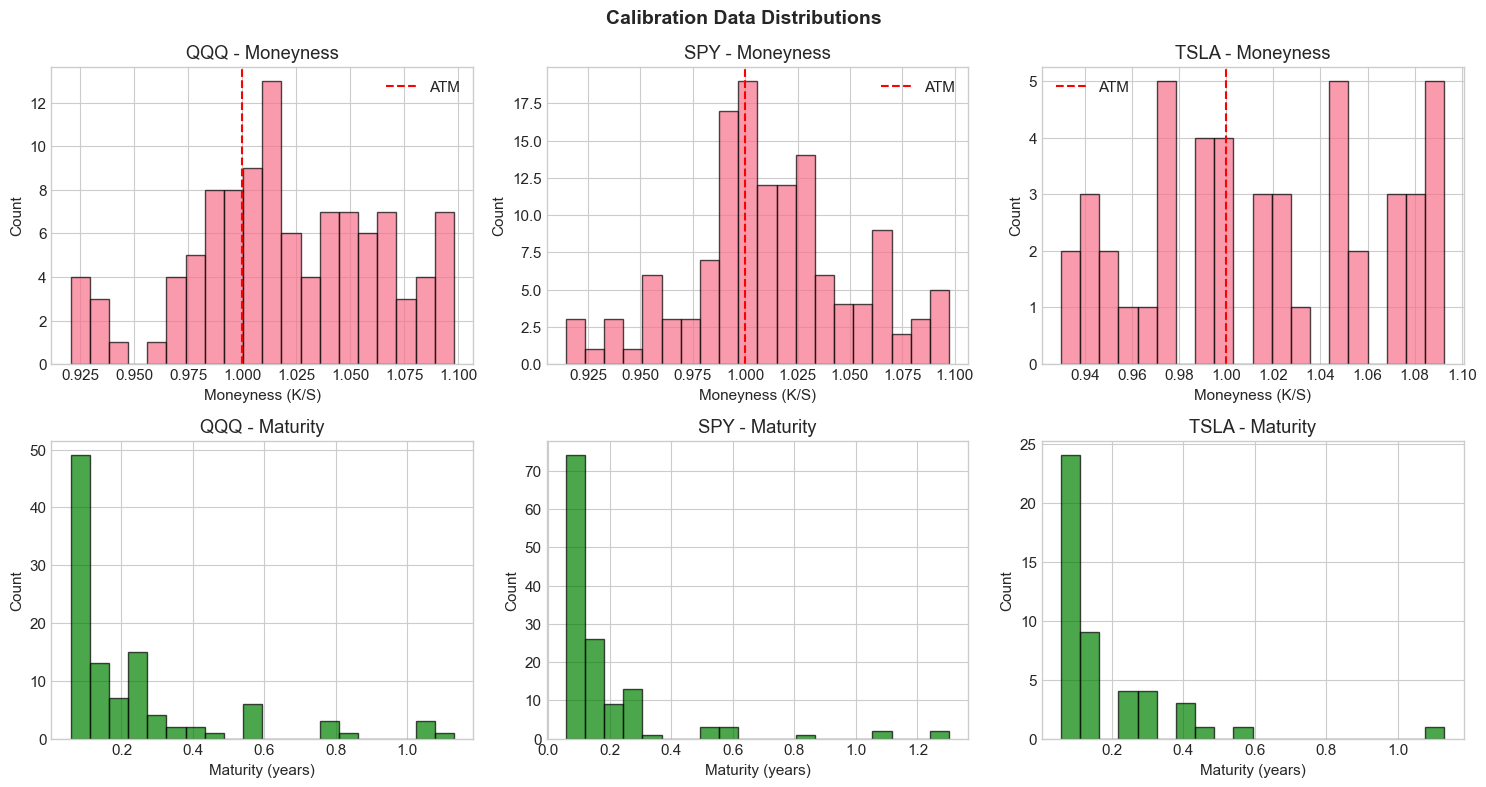
\includegraphics[width=0.9\textwidth]{figures/data_collection.png}
        \caption{End-to-end data collection and preprocessing pipeline}
    \end{figure}
\end{frame}

\subsection{Neural Network Architecture}

\begin{frame}{Heston Surrogate Network}
    \begin{figure}
        \centering
        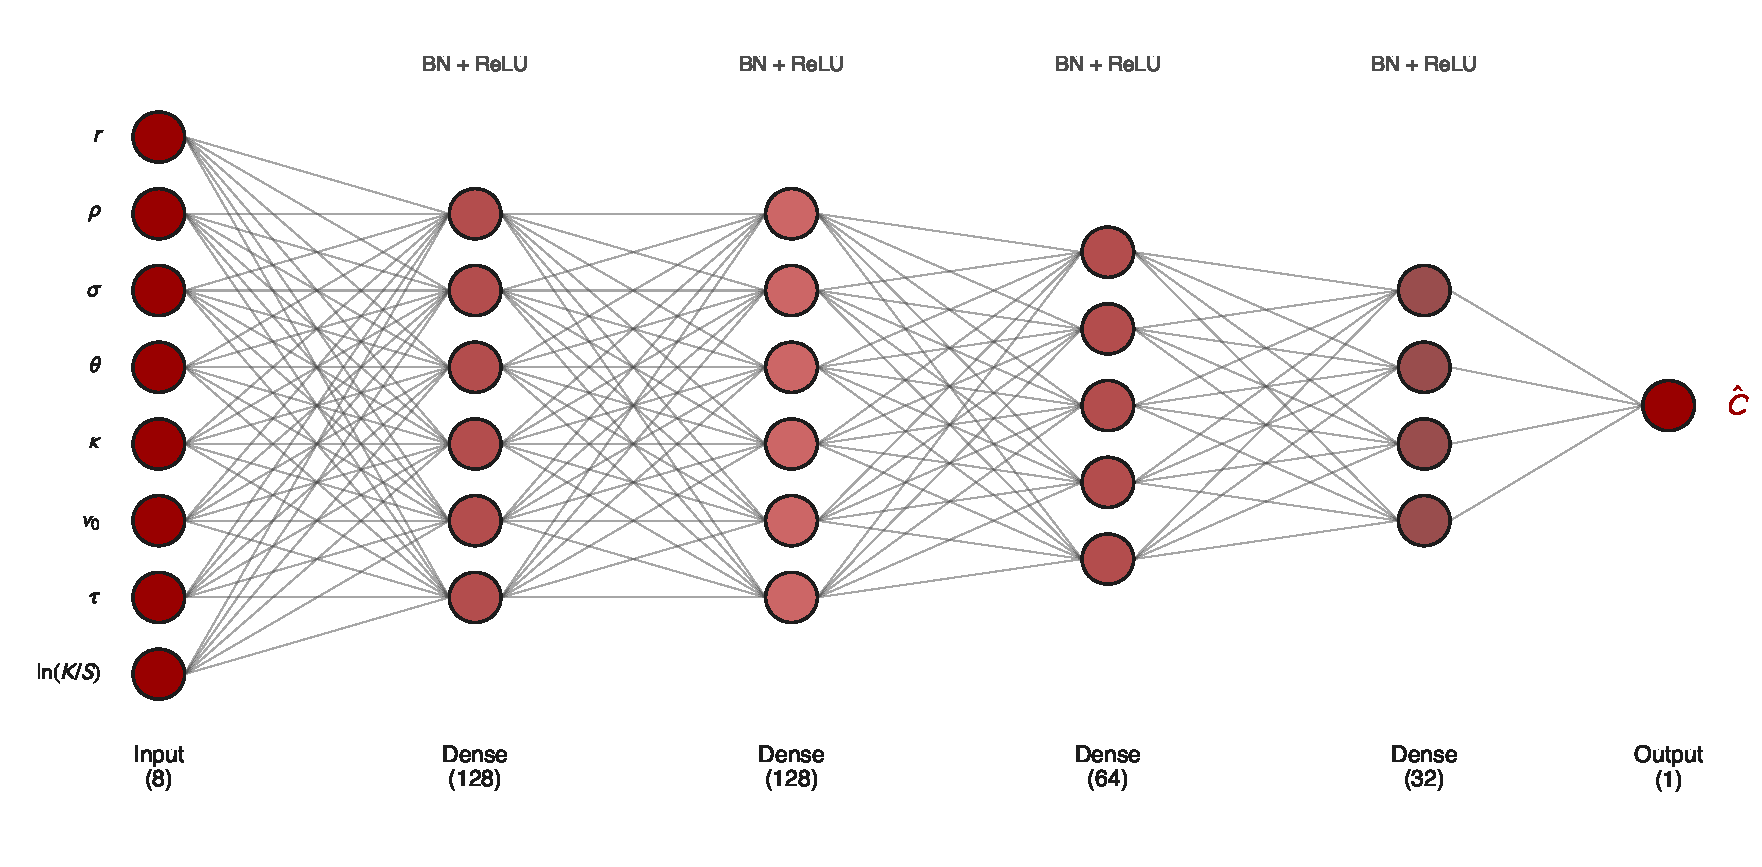
\includegraphics[width=0.85\textwidth]{figures/nn_architecture.pdf}
        \caption{Neural network architecture for Heston price approximation}
    \end{figure}
\end{frame}

\begin{frame}{Network Architecture}
    \begin{block}{Input Layer: 8 Features}
        \begin{columns}
            \begin{column}{0.5\textwidth}
                \textbf{Option Characteristics:}
                \begin{itemize}
                    \item Log-moneyness: $\ln(K/S)$
                    \item Time to maturity: $T$
                    \item Risk-free rate: $r$
                \end{itemize}
            \end{column}
            \begin{column}{0.5\textwidth}
                \textbf{Heston Parameters:}
                \begin{itemize}
                    \item Initial variance: $v_0$
                    \item Mean reversion: $\kappa$, $\theta$
                    \item Vol-of-vol: $\sigma$, Correlation: $\rho$
                \end{itemize}
            \end{column}
        \end{columns}
    \end{block}

    \begin{block}{Hidden Layers: [128, 128, 64, 32]}
        \begin{itemize}
            \item \textbf{LeakyReLU} ($\alpha=0.1$): avoids dying neurons
            \item \textbf{Batch Norm} + \textbf{Dropout} (10\%) for regularization
        \end{itemize}
    \end{block}

    \begin{alertblock}{Output Layer}
        \textbf{Softplus}: $f(x) = \ln(1 + e^x)$ ensures $C > 0$
    \end{alertblock}
\end{frame}

\begin{frame}{Training Configuration}
    \begin{columns}
        \begin{column}{0.5\textwidth}
            \begin{block}{Data Generation}
                \begin{itemize}
                    \item \textbf{100,000} synthetic samples
                    \item Security-specific parameter ranges
                    \item Importance sampling: 60\% Gaussian, 70\% ATM
                \end{itemize}
            \end{block}
        \end{column}
        \begin{column}{0.5\textwidth}
            \begin{block}{Optimization}
                \begin{itemize}
                    \item Adam ($\eta=10^{-3}$), weight decay $10^{-5}$
                    \item Loss: MSE on normalized prices
                    \item Max epochs: 200
                \end{itemize}
            \end{block}
        \end{column}
    \end{columns}

    \vspace{0.2cm}

    \begin{block}{Learning Rate Schedule}
        \textbf{ReduceLROnPlateau:} Reduce $\eta$ by 50\% after 10 epochs plateau.
        \textbf{Early Stopping:} Patience 25 epochs, restore best weights.
    \end{block}
\end{frame}

\subsection{Calibration Methods}

\begin{frame}{Calibration Problem Formulation}
    \begin{block}{Objective: Minimize Pricing Error}
        Find Heston parameters $\Theta = (v_0, \kappa, \theta, \sigma, \rho)$ that minimize:
        \begin{equation}
            \mathcal{L}(\Theta) = \sum_{i=1}^N \left(C_i^{\text{market}} - C_i^{\text{model}}(\Theta)\right)^2
        \end{equation}
    \end{block}

    \vspace{0.2cm}

    \begin{columns}
        \begin{column}{0.5\textwidth}
            \begin{block}{Traditional (FFT)}
                $C_i^{\text{model}} = C_i^{\text{FFT}}(\Theta)$
                \begin{itemize}
                    \item Carr-Madan FFT pricing
                    \item SLSQP (gradient-based)
                    \item Tol: $10^{-8}$, 500 iter
                \end{itemize}
            \end{block}
        \end{column}
        \begin{column}{0.5\textwidth}
            \begin{block}{NN Surrogate}
                $C_i^{\text{model}} = S_0 \cdot \mathcal{N}_\theta(\Theta, m_i, \tau_i, r_i)$
                \begin{itemize}
                    \item Trained neural network
                    \item Diff. Evolution (global)
                    \item 200 iter, population
                \end{itemize}
            \end{block}
        \end{column}
    \end{columns}
\end{frame}

\begin{frame}{Fair Comparison Framework}
    \begin{block}{Why Different Optimizers?}
        Each method uses its \textbf{optimal} algorithm to isolate pricing function performance:
    \end{block}

    \begin{columns}
        \begin{column}{0.5\textwidth}
            \textbf{FFT + SLSQP:}
            \begin{itemize}
                \item FFT is smooth, differentiable
                \item SLSQP exploits local structure
                \item Fast convergence near optimum
            \end{itemize}
        \end{column}
        \begin{column}{0.5\textwidth}
            \textbf{NN + Differential Evolution:}
            \begin{itemize}
                \item NN may have irregularities
                \item DE robust to noise
                \item Global search avoids local minima
            \end{itemize}
        \end{column}
    \end{columns}

    \vspace{0.2cm}

    \begin{alertblock}{Security-Specific Bounds}
        Parameter ranges from historical volatility: $v_0, \theta$ from realized vol, $\rho$ from leverage.
    \end{alertblock}
\end{frame}

%===========================================
% SECTION 4: RESULTS
%===========================================
\section{Results}

\subsection{Performance Comparison}

\begin{frame}{Key Performance Metrics}
    \begin{figure}
        \centering
        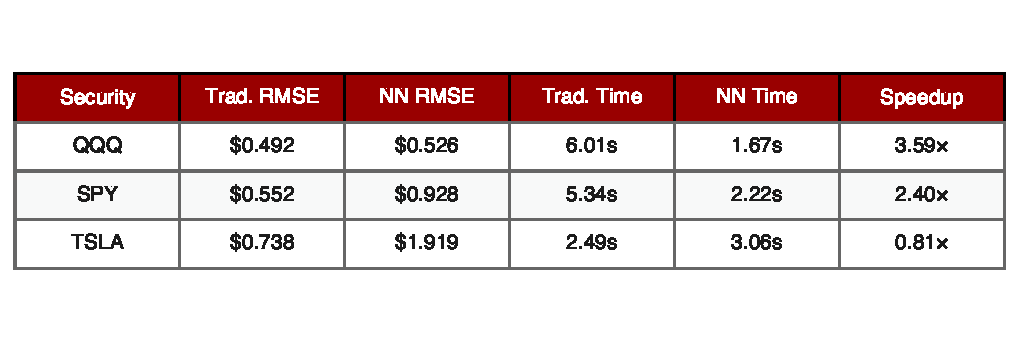
\includegraphics[width=0.9\textwidth]{figures/performance_summary_table.pdf}
        \caption{Summary of calibration performance: Traditional FFT vs Neural Network}
    \end{figure}
\end{frame}

\begin{frame}{Calibration Time and Pricing Accuracy}
    \begin{figure}
        \centering
        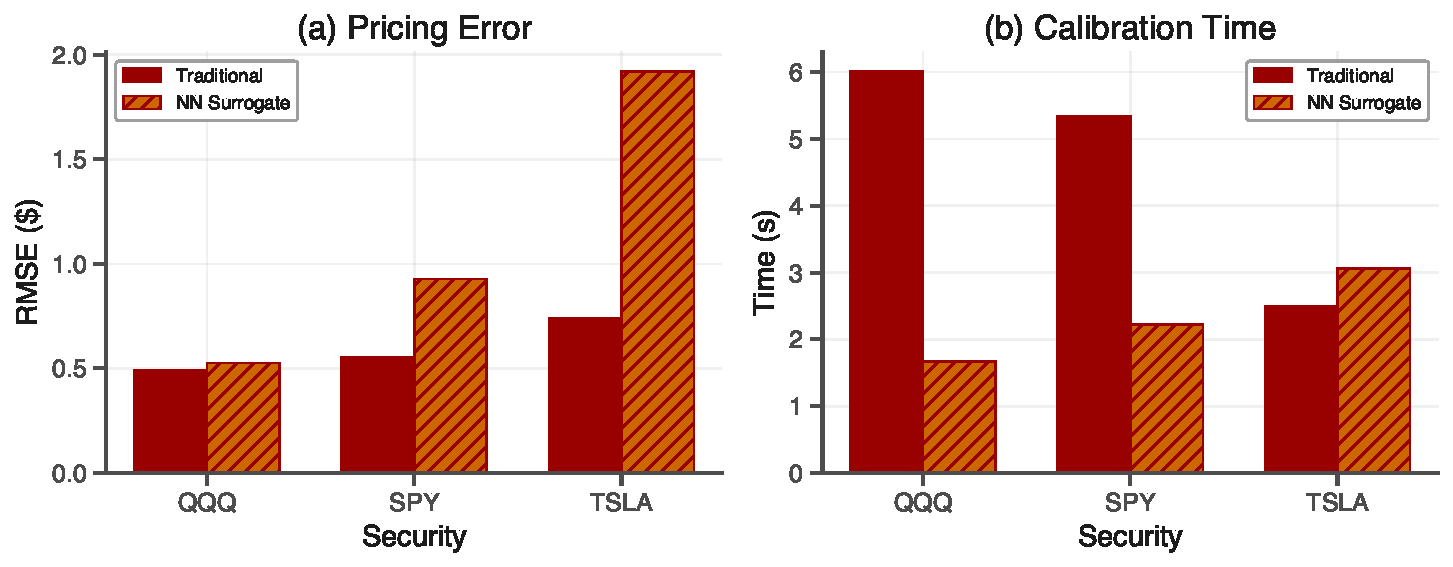
\includegraphics[width=0.8\textwidth]{figures/combined_performance.pdf}
        \caption{Calibration time and pricing accuracy comparison: FFT vs Neural Network}
    \end{figure}
\end{frame}

\begin{frame}{Speedup Analysis}
    \begin{figure}
        \centering
        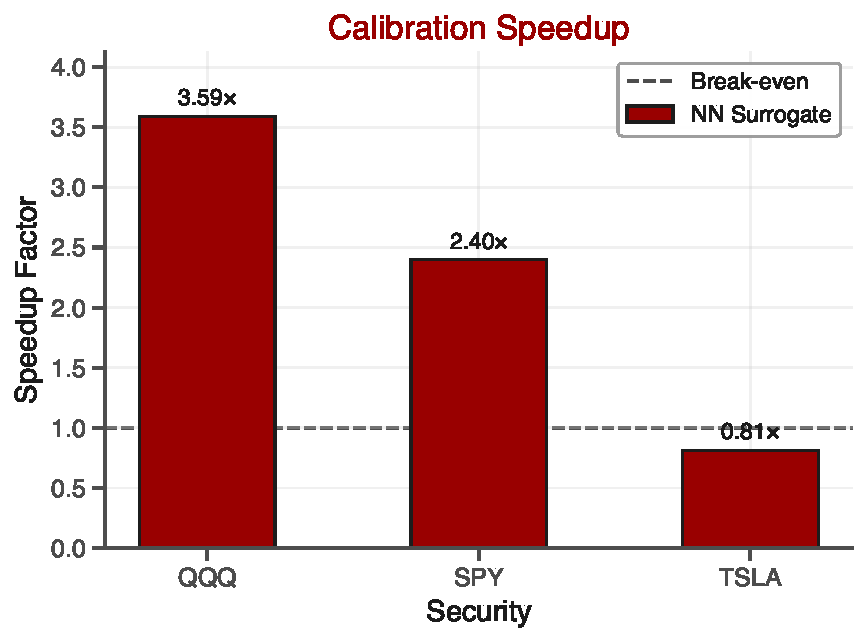
\includegraphics[width=0.8\textwidth]{figures/speedup_comparison.pdf}
        \caption{Calibration speedup vs traditional FFT method}
    \end{figure}
\end{frame}

\begin{frame}{Neural Network Performance: Market vs Model}
    \begin{figure}
        \centering
        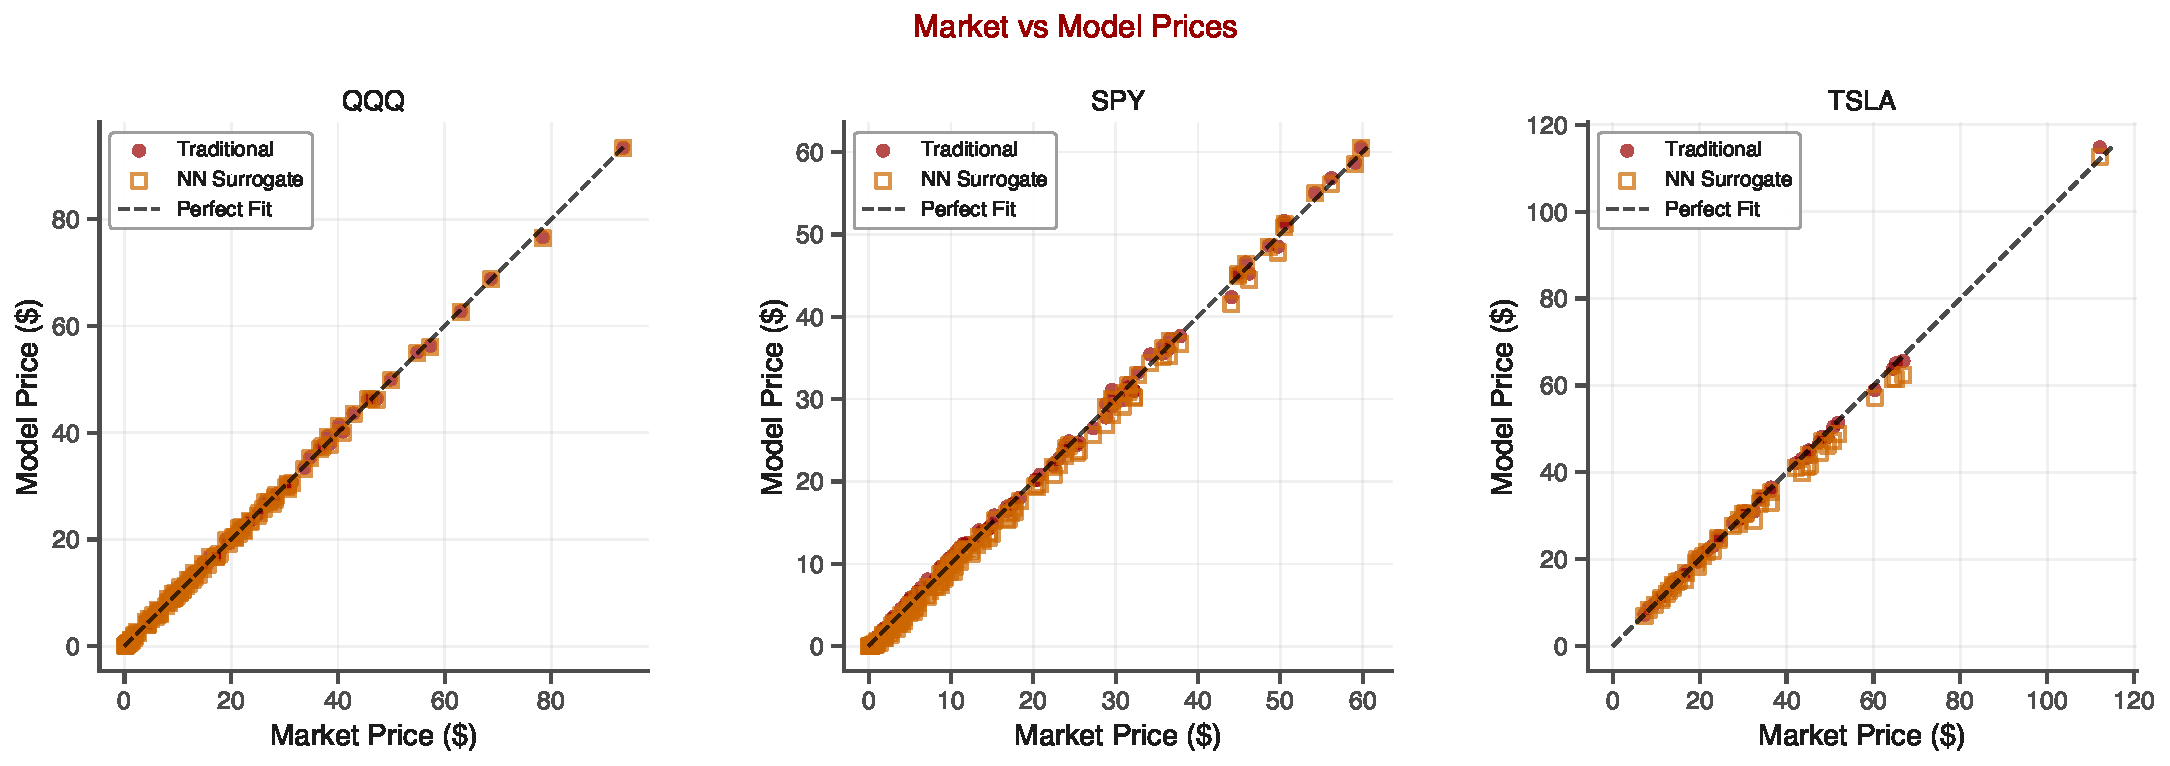
\includegraphics[width=0.95\textwidth]{figures/market_vs_model_prices.pdf}
        \caption{Comparison of market prices vs model predictions by calibration method}
    \end{figure}
\end{frame}

\begin{frame}{Neural Network Performance: Error Analysis}
    \begin{figure}
        \centering
        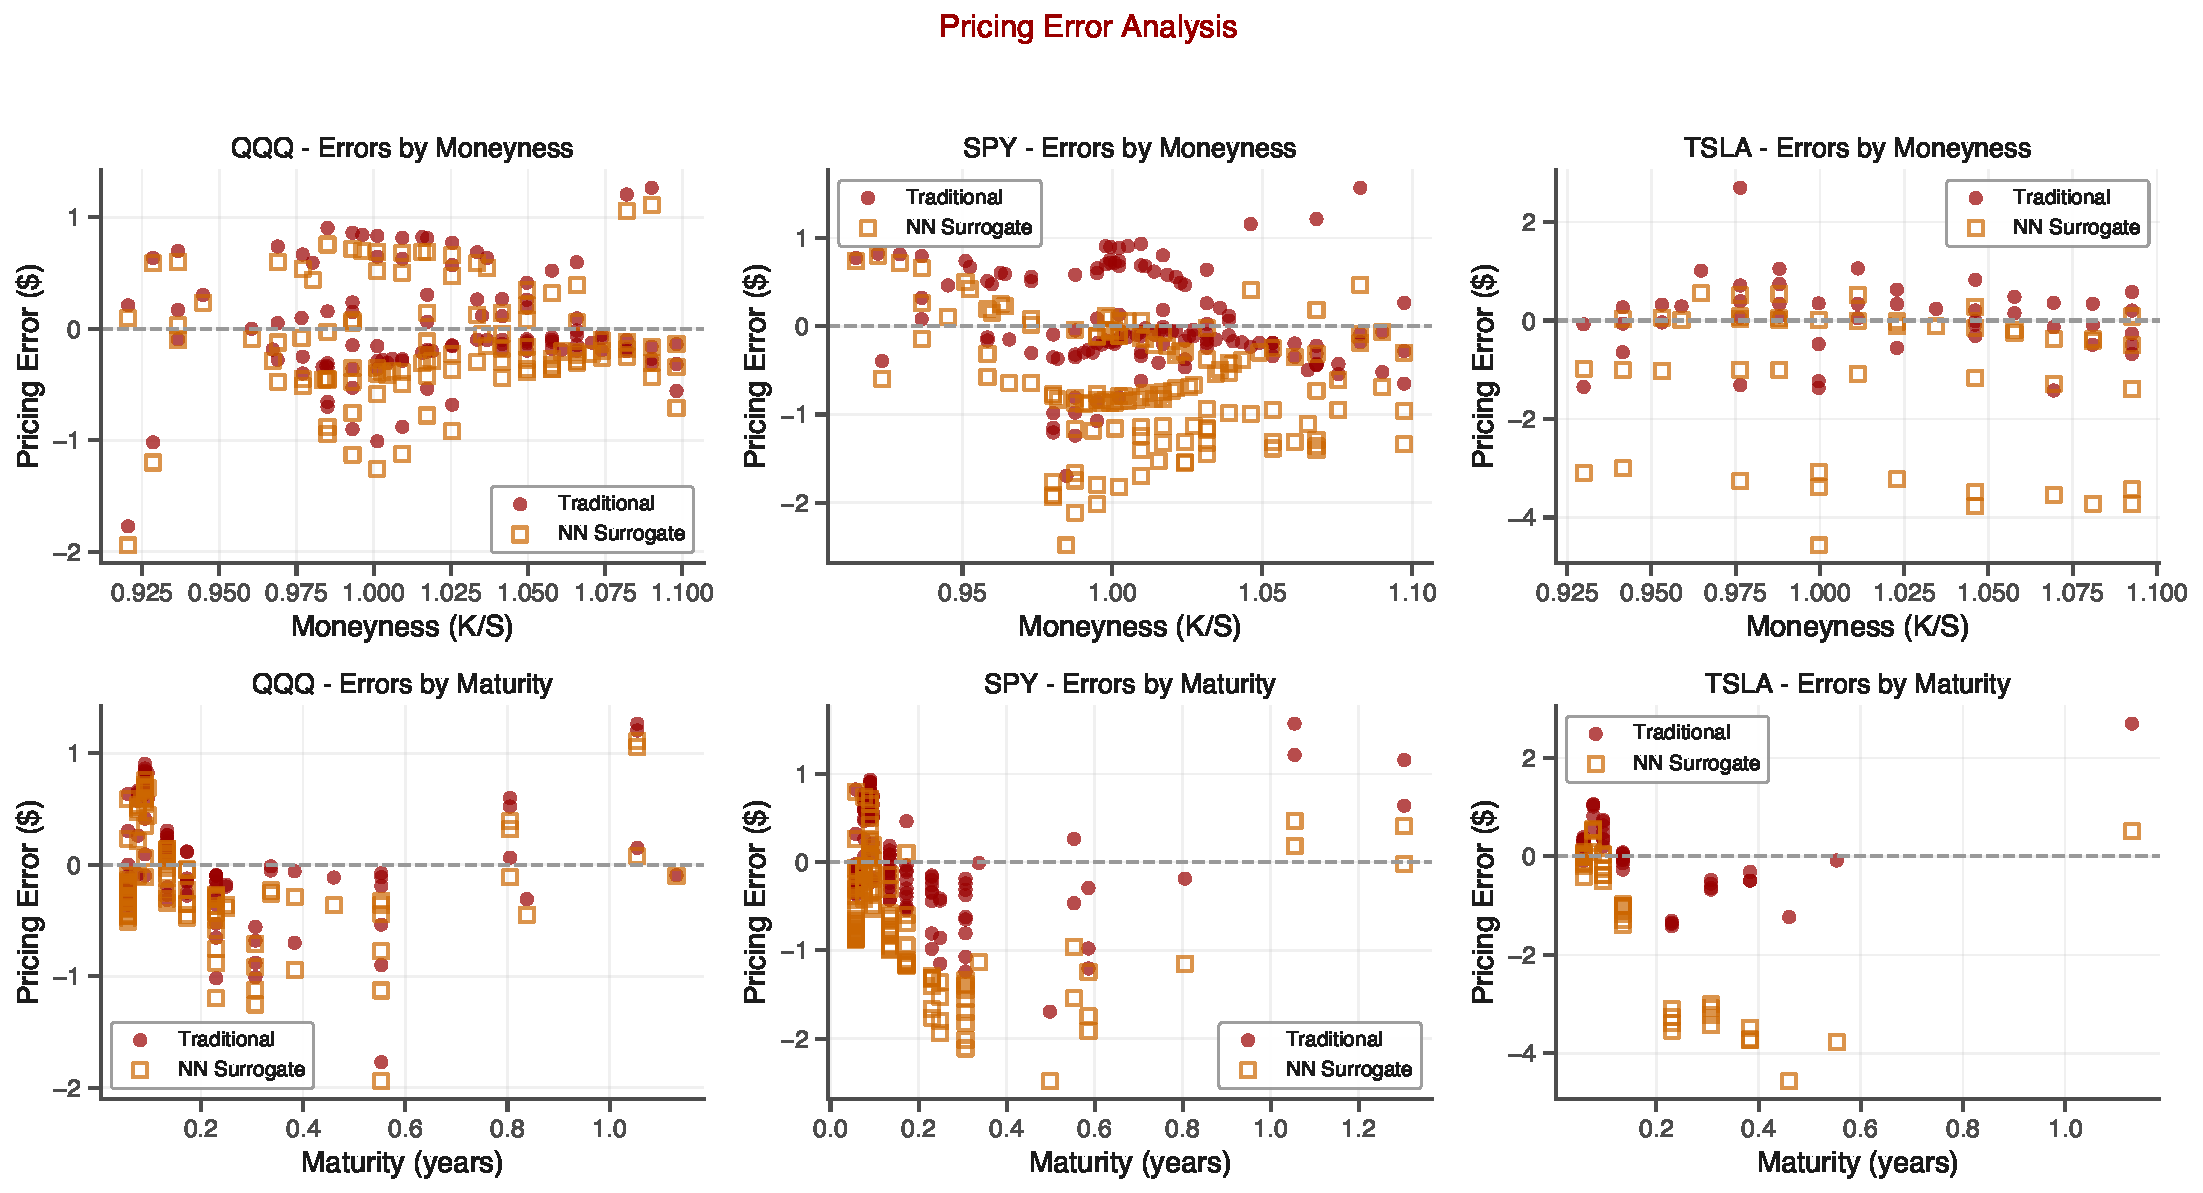
\includegraphics[width=0.95\textwidth]{figures/error_analysis.pdf}
        \caption{Pricing errors by moneyness and maturity dimensions}
    \end{figure}
\end{frame}

\begin{frame}{Trade-off Analysis}
    \begin{figure}
        \centering
        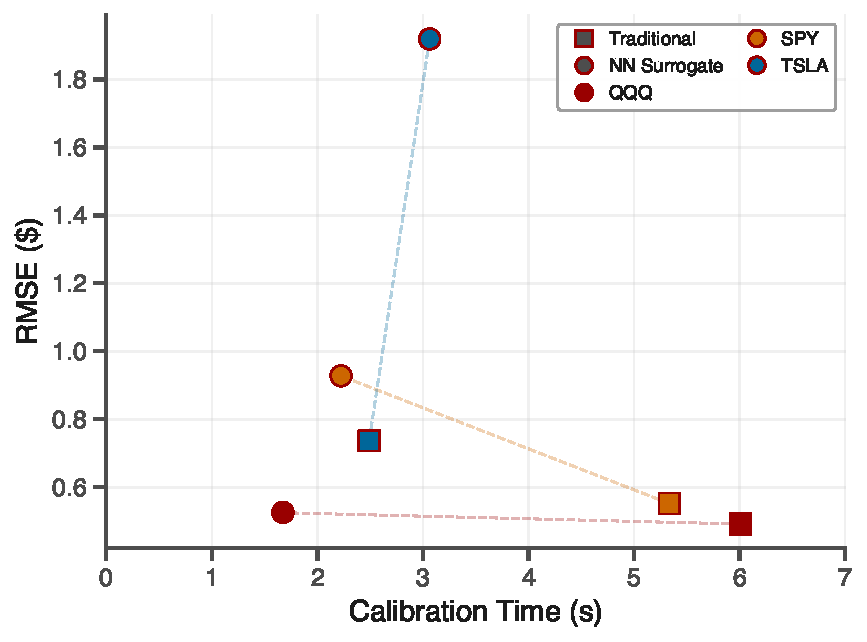
\includegraphics[width=0.85\textwidth]{figures/accuracy_speed_tradeoff.pdf}
        \caption{Accuracy vs speed trade-off across securities}
    \end{figure}
\end{frame}

\subsection{Parameter Recovery}

\begin{frame}{Calibrated Heston Parameters}
    \begin{figure}
        \centering
        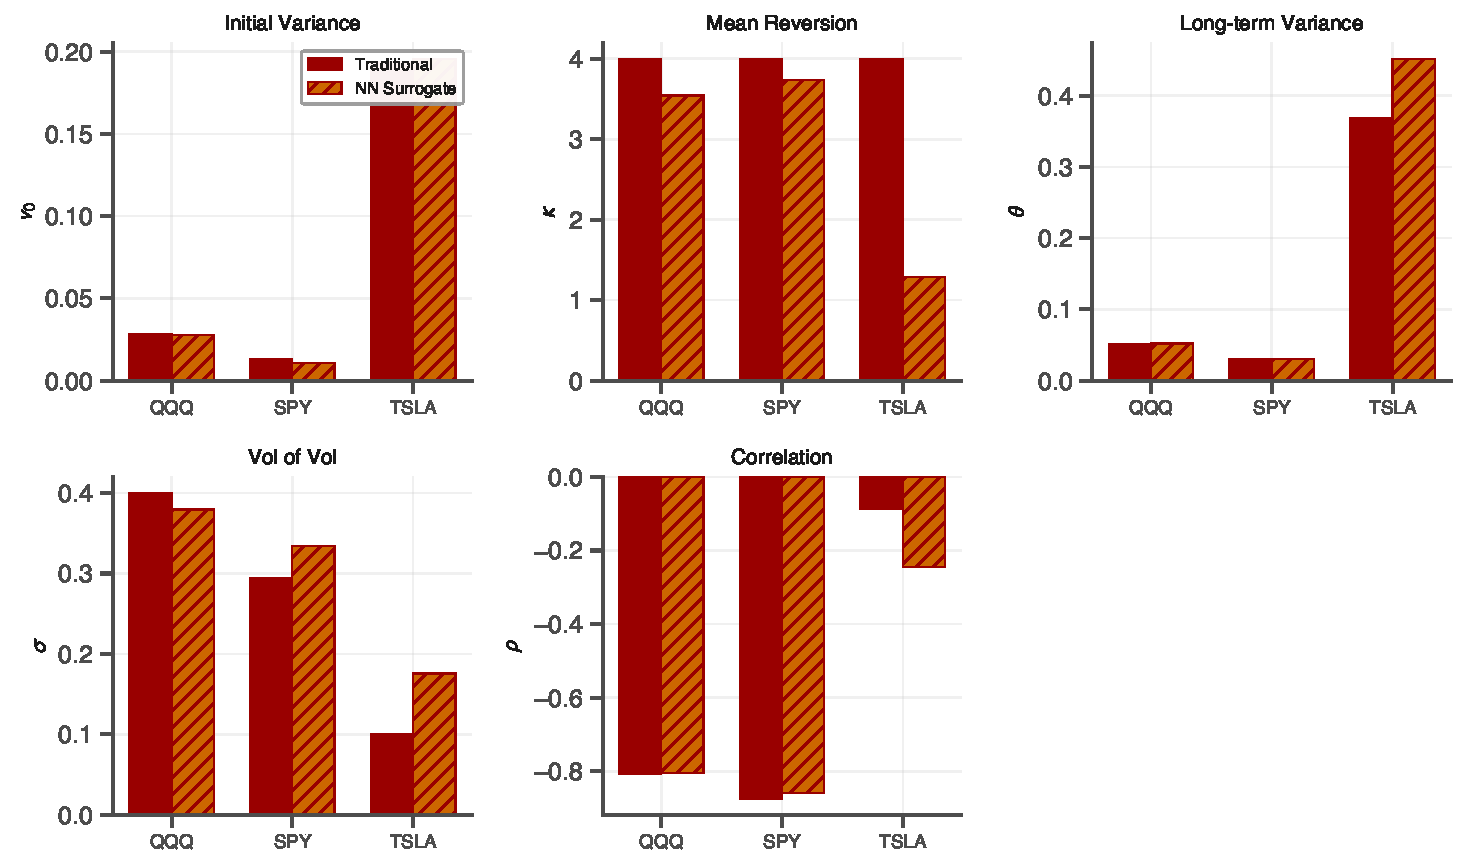
\includegraphics[width=0.95\textwidth]{figures/parameter_comparison_detailed.pdf}
        \caption{Comparison of calibrated Heston parameters}
    \end{figure}
\end{frame}

\subsection{Statistical Assessment}

\begin{frame}{Robustness Assessment: Hypothesis Testing and Effect Sizes}
    \begin{figure}
        \centering
        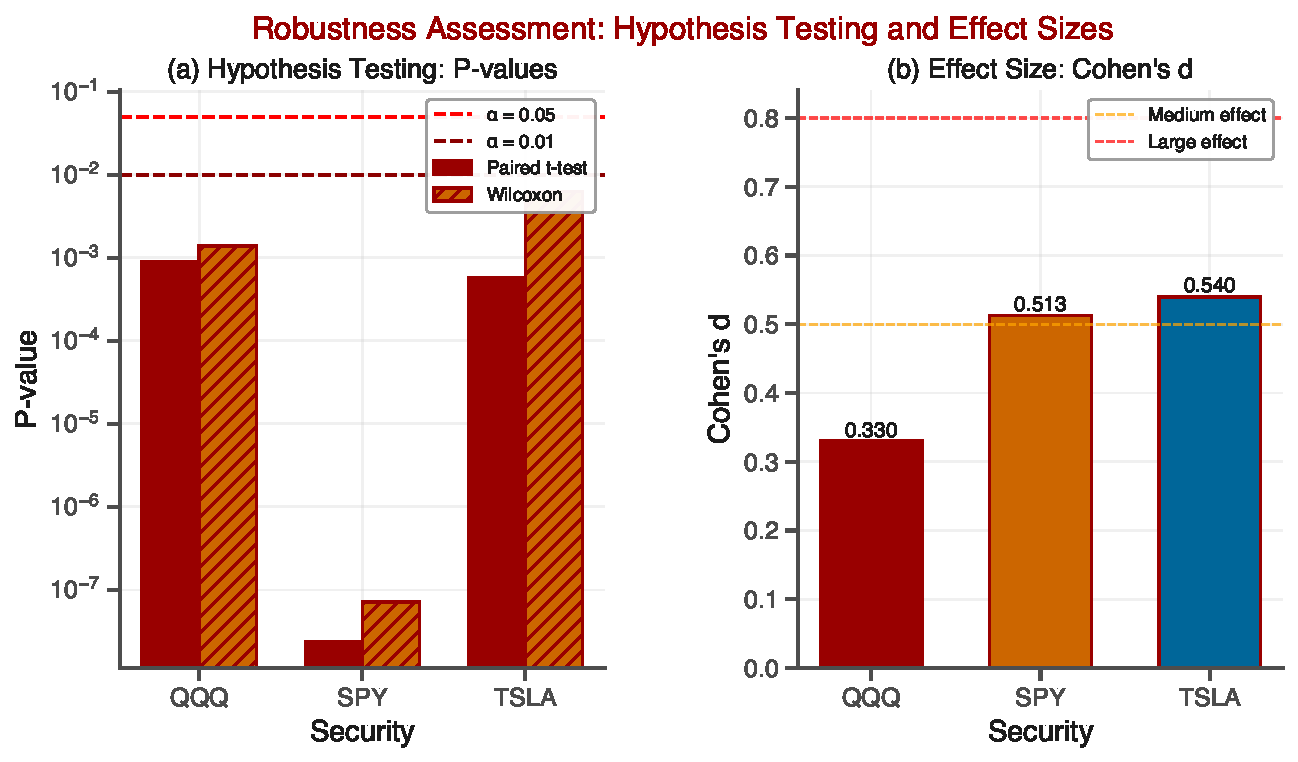
\includegraphics[width=0.75\textwidth]{figures/robustness_hypothesis_effect.pdf}
        \caption{Hypothesis testing (p-values) and effect size analysis (Cohen's d, Glass's $\Delta$, Hedges' g)}
    \end{figure}

    \tiny
    Significant differences (p < 0.01) for all securities. Medium effect sizes (Cohen's d: 0.33--0.54) indicate practical significance.
\end{frame}

\begin{frame}{Robustness Assessment: Normality Tests and Confidence Intervals}
    \begin{figure}
        \centering
        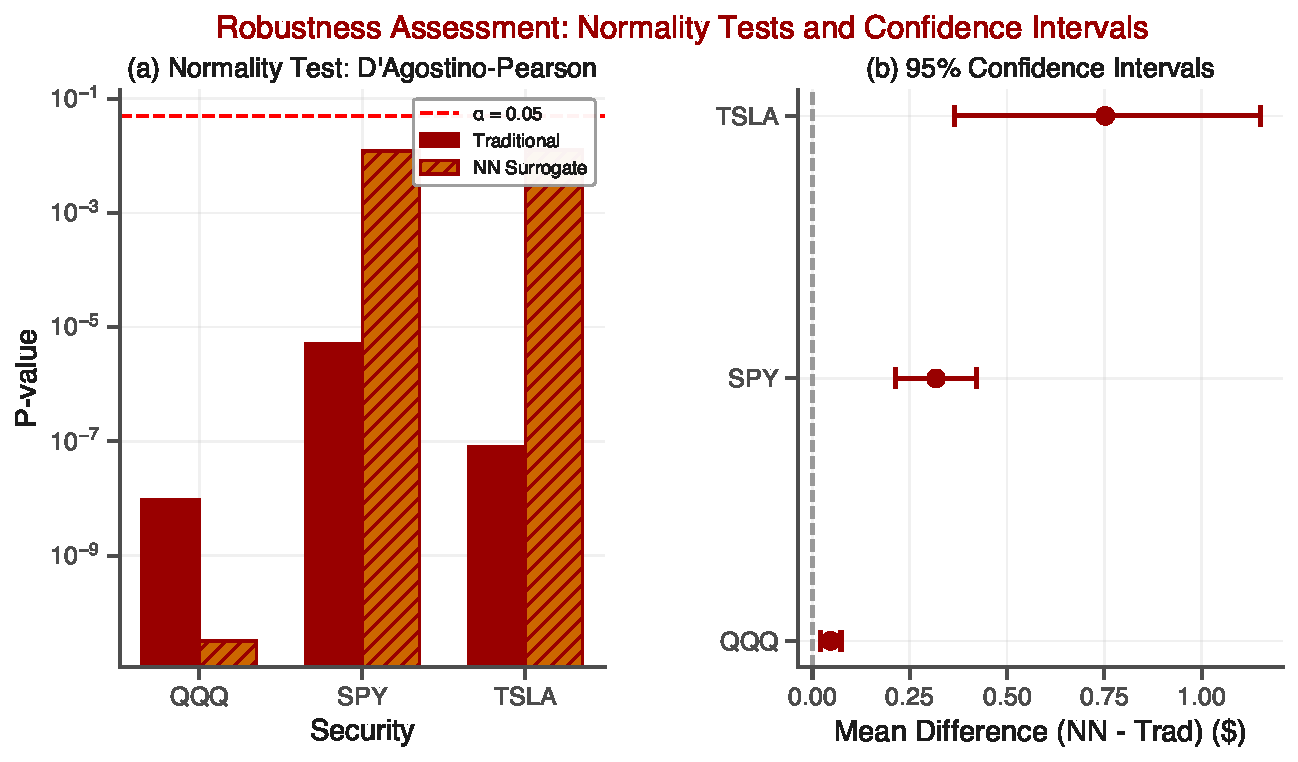
\includegraphics[width=0.75\textwidth]{figures/robustness_normality_ci.pdf}
        \caption{Normality tests and confidence intervals}
    \end{figure}

    \tiny
    Errors are non-normal (p < 0.05), justifying non-parametric tests. Confidence intervals do not contain zero, confirming significant differences.
\end{frame}

%===========================================
% SECTION 5: DISCUSSION
%===========================================
\section{Discussion}

\begin{frame}{Key Findings}
    \begin{block}{Performance Summary}
        \centering
        \small
        \begin{tabular}{lccc}
            \toprule
            \textbf{Security} & \textbf{Speedup} & \textbf{RMSE $\Delta$} & \textbf{Verdict} \\
            \midrule
            QQQ & \textcolor{green!60!black}{3.6$\times$} & \textcolor{green!60!black}{+7\%} & \checkmark Excellent \\
            SPY & \textcolor{orange!80!black}{2.4$\times$} & \textcolor{orange!80!black}{+68\%} & $\sim$ Acceptable \\
            TSLA & \textcolor{red!80!black}{0.8$\times$} & \textcolor{red!80!black}{+160\%} & $\times$ Not suitable \\
            \bottomrule
        \end{tabular}
    \end{block}

    \vspace{0.2cm}

    \begin{columns}
        \begin{column}{0.5\textwidth}
            \begin{alertblock}{Key Insight}
                NN performance correlates with volatility regime
            \end{alertblock}
        \end{column}
        \begin{column}{0.5\textwidth}
            \begin{exampleblock}{Recommendation}
                Deploy for moderate-volatility assets
            \end{exampleblock}
        \end{column}
    \end{columns}
\end{frame}

\begin{frame}{Limitations \& Future Work}
    \begin{columns}
        \begin{column}{0.5\textwidth}
            \begin{block}{Current Limitations}
                \small
                \begin{itemize}
                    \item Security-specific training
                    \item High-volatility degradation
                    \item Parameter range sensitivity
                    \item Single-day evaluation
                    \item No uncertainty quantification
                \end{itemize}
            \end{block}
        \end{column}
        \begin{column}{0.5\textwidth}
            \begin{block}{Future Directions}
                \small
                \begin{itemize}
                    \item Transfer learning
                    \item Ensemble methods
                    \item Bayesian NNs for uncertainty
                    \item Exotic options extension
                    \item Multi-period analysis
                \end{itemize}
            \end{block}
        \end{column}
    \end{columns}
\end{frame}

%===========================================
% SECTION 6: CONCLUSION
%===========================================
\section{Conclusion}

\begin{frame}{Conclusions}
    \begin{block}{Research Contributions}
        \begin{enumerate}
            \item Demonstrated neural network surrogates can accelerate Heston calibration by up to \textbf{3.6$\times$}
            \item Documented substantial \textbf{performance heterogeneity} across volatility regimes
            \item Provided \textbf{evidence-based deployment criteria} for practitioners
            \item Established rigorous benchmarking methodology with fair comparison
        \end{enumerate}
    \end{block}

    \vspace{0.3cm}

    \begin{alertblock}{Practical Implications}
        Neural network calibration is most effective for:
        \begin{itemize}
            \item Liquid securities with moderate volatility
            \item Applications tolerating small accuracy trade-offs
            \item High-frequency calibration requirements
        \end{itemize}
    \end{alertblock}
\end{frame}

\begin{frame}{Summary Statistics}
    \centering
    \begin{tabular}{lcc}
        \toprule
        \textbf{Metric} & \textbf{Average} & \textbf{Best (QQQ)} \\
        \midrule
        Speedup Factor & 2.27$\times$ & 3.59$\times$ \\
        RMSE Increase & 78\% & 7\% \\
        Traditional Time & 4.6s & 6.0s \\
        NN Time & 2.3s & 1.7s \\
        \bottomrule
    \end{tabular}

    \vspace{1cm}

    \begin{block}{Bottom Line}
        Neural network surrogate models offer a viable path to faster option pricing model calibration, with performance depending critically on underlying security characteristics.
    \end{block}
\end{frame}

%===========================================
% REFERENCES
%===========================================
\section{References}

\begin{frame}[allowframebreaks]{References}
    \nocite{heston1993, black1973, hutchinson1994, liu2019, HorvathMuguruzaTomas2019, carr1999, cont2004, Rubinstein1985, Lamoureux1993, Black1976}
    \bibliographystyle{ieeetr}
    \bibliography{ref}
\end{frame}

%===========================================
% THANK YOU
%===========================================
\begin{frame}
    \begin{center}
        {\Huge\calligra Thank You}

        \vspace{1cm}

        \textbf{Questions?}

        \vspace{1cm}

        \small
        Joris Marvezy \\
        TBS Education \\
        December 2025
    \end{center}
\end{frame}

%===========================================
% APPENDIX
%===========================================
\appendix

%-------------------------------------------
% APPENDIX SECTION: Training Details
%-------------------------------------------
\begin{frame}
    \begin{center}
        \vspace{2cm}
        {\LARGE \textbf{Appendix A}}\\[0.5cm]
        {\Large Training Details}\\[1cm]
        \textit{Neural Network Training Convergence and Configuration}
    \end{center}
\end{frame}

\begin{frame}{Training Convergence}
    \begin{figure}
        \centering
        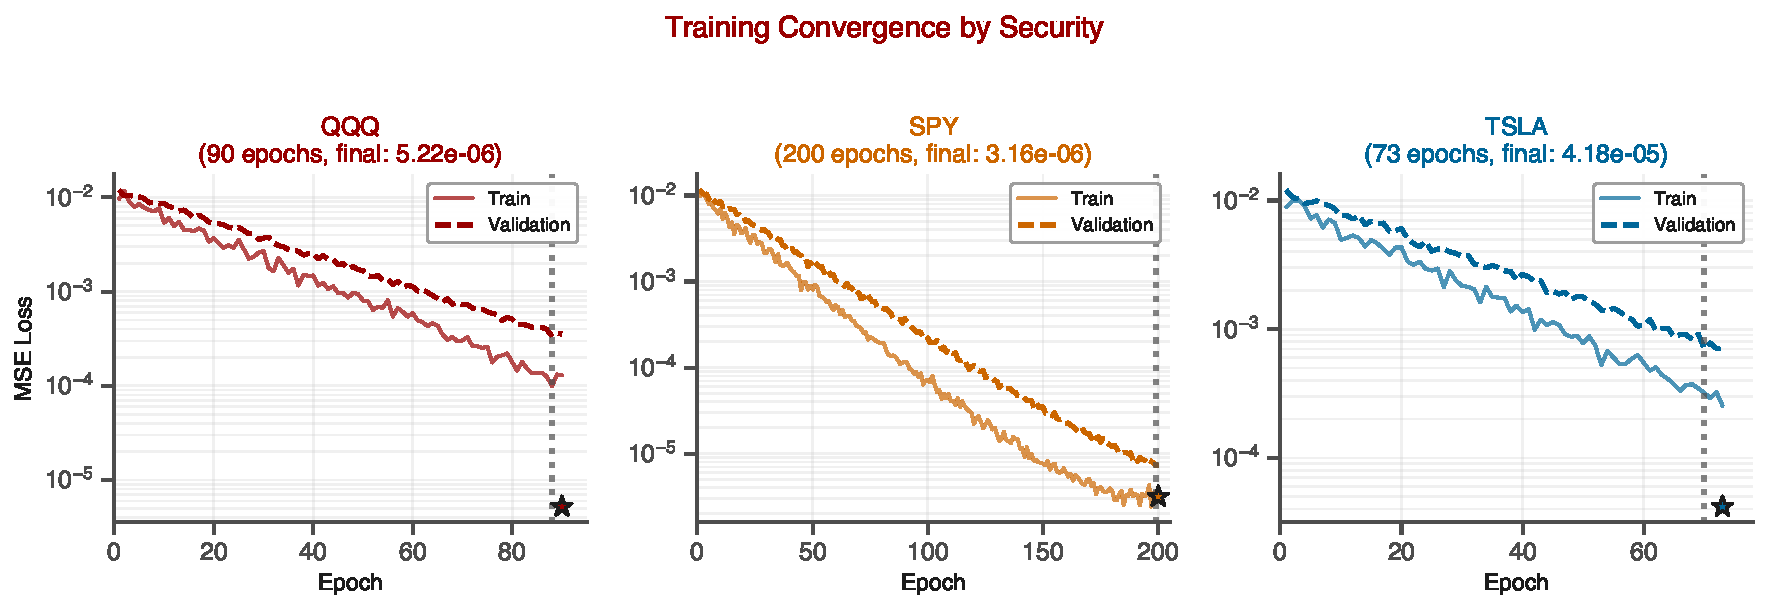
\includegraphics[width=0.95\textwidth]{figures/training_convergence.pdf}
        \caption{Training and validation loss curves for each security}
    \end{figure}
\end{frame}

\begin{frame}{Training Configuration}
    \begin{columns}
        \begin{column}{0.5\textwidth}
            \begin{block}{Early Stopping}
                \begin{itemize}
                    \item Patience: 25 epochs
                    \item Validation split: 20\%
                    \item Best checkpoint saved
                \end{itemize}
            \end{block}
        \end{column}
        \begin{column}{0.5\textwidth}
            \begin{block}{Convergence Results}
                \small
                \begin{tabular}{lcc}
                    \toprule
                    \textbf{Ticker} & \textbf{Epochs} & \textbf{Val Loss} \\
                    \midrule
                    QQQ & 90 & $5.2 \times 10^{-6}$ \\
                    SPY & 200 & $3.2 \times 10^{-6}$ \\
                    TSLA & 73 & $4.2 \times 10^{-5}$ \\
                    \bottomrule
                \end{tabular}
            \end{block}
        \end{column}
    \end{columns}
\end{frame}

\begin{frame}{Neural Network Training Process}
    \begin{figure}
        \centering
        \animategraphics[loop,autoplay,controls,width=0.90\textwidth]{20}{figures/nn_training_frames/nn_training_animation_}{000}{299}
        \caption{Training progress: QQQ network training (90 epochs, final loss: $5.22 \times 10^{-6}$)}
    \end{figure}
\end{frame}

%-------------------------------------------
% APPENDIX SECTION: Technical Background
%-------------------------------------------
\begin{frame}
    \begin{center}
        \vspace{2cm}
        {\LARGE \textbf{Appendix B}}\\[0.5cm]
        {\Large Technical Background}\\[1cm]
        \textit{Neural Networks, Optimization, and Model Theory}
    \end{center}
\end{frame}

\begin{frame}{Neural Network Fundamentals}
    \begin{block}{Universal Approximation Theorem}
        A feedforward network with sufficient neurons can approximate any continuous function on compact subsets of $\mathbb{R}^n$ to arbitrary precision.
    \end{block}

    \vspace{0.3cm}

    \begin{columns}
        \begin{column}{0.5\textwidth}
            \textbf{Key Components:}
            \begin{itemize}
                \item \textbf{LeakyReLU:} $f(x) = \max(\alpha x, x)$
                \item \textbf{Batch Normalization}
                \item \textbf{Dropout:} 10\%
                \item \textbf{Softplus output:} $C > 0$
            \end{itemize}
        \end{column}
        \begin{column}{0.5\textwidth}
            \textbf{Why Feedforward?}
            \begin{itemize}
                \item Simple, fast inference
                \item Well-understood behavior
                \item Sufficient for static mapping
                \item Easy production deployment
            \end{itemize}
        \end{column}
    \end{columns}
\end{frame}

\begin{frame}{Activation Functions in Detail}
    \small
    \begin{columns}
        \begin{column}{0.5\textwidth}
            \begin{block}{LeakyReLU (Hidden)}
                \begin{equation}
                    f(x) = \begin{cases} x & x > 0 \\ \alpha x & x \leq 0 \end{cases}
                \end{equation}
                \begin{itemize}
                    \item $\alpha = 0.1$ (leak coefficient)
                    \item Avoids dying ReLU problem
                \end{itemize}
            \end{block}
        \end{column}
        \begin{column}{0.5\textwidth}
            \begin{block}{Softplus (Output)}
                \begin{equation}
                    f(x) = \ln(1 + e^x)
                \end{equation}
                \begin{itemize}
                    \item Smooth approximation to ReLU
                    \item Ensures $C > 0$ (positive prices)
                \end{itemize}
            \end{block}
        \end{column}
    \end{columns}

    \begin{block}{Batch Normalization}
        Normalizes inputs: $\hat{x} = \frac{x - \mu}{\sqrt{\sigma^2 + \epsilon}}$, then scales/shifts. Stabilizes training.
    \end{block}
\end{frame}

\begin{frame}{Statistical Testing Framework}
    \begin{block}{Hypothesis Testing}
        \begin{itemize}
            \item \textbf{Null hypothesis:} No difference in RMSE between methods
            \item \textbf{Test:} Two-sample t-test (paired)
            \item \textbf{Correction:} Bonferroni ($\alpha_{\text{adj}} = 0.05/3 = 0.0167$)
        \end{itemize}
    \end{block}

    \vspace{0.3cm}

    \begin{block}{Effect Size Interpretation (Cohen's $d$)}
        \centering
        \begin{tabular}{lc}
            \toprule
            \textbf{Effect Size} & \textbf{Cohen's $d$} \\
            \midrule
            Negligible & $|d| < 0.2$ \\
            Small & $0.2 \leq |d| < 0.5$ \\
            Medium & $0.5 \leq |d| < 0.8$ \\
            Large & $|d| \geq 0.8$ \\
            \bottomrule
        \end{tabular}
    \end{block}
\end{frame}

\begin{frame}{Feller Condition}
    \begin{block}{Model Stability Requirement}
        The variance process remains strictly positive if:
        \begin{equation}
            2\kappa\theta \geq \sigma^2
        \end{equation}
        This prevents variance from hitting zero (non-physical).
    \end{block}

    \vspace{0.3cm}

    \begin{block}{Parameter Interpretation}
        \begin{itemize}
            \item $\kappa$ large: Fast mean reversion to $\theta$
            \item $\sigma$ large: High volatility-of-volatility
            \item $\rho < 0$: Leverage effect (prices fall $\rightarrow$ vol rises)
            \item Typical equity $\rho$: $-0.3$ to $-0.8$
        \end{itemize}
    \end{block}
\end{frame}

\begin{frame}{Synthetic Data Generation}
    \begin{block}{Importance Sampling Strategy}
        Training data concentrated where it matters:
        \begin{itemize}
            \item \textbf{60\%} truncated Gaussian (likely parameter regions)
            \item \textbf{40\%} uniform distribution (tail coverage)
            \item \textbf{70\%} ATM options (moneyness $\in [0.95, 1.05]$)
            \item \textbf{30\%} full moneyness range $[0.90, 1.10]$
        \end{itemize}
    \end{block}

    \vspace{0.3cm}

    \begin{block}{Security-Specific Ranges}
        Historical volatility statistics inform parameter bounds:
        \begin{itemize}
            \item $v_0, \theta$ from realized volatility
            \item $\rho$ from leverage correlation
            \item Avoids generic ranges that waste capacity
        \end{itemize}
    \end{block}
\end{frame}

\begin{frame}{Security-Specific Parameter Bounds}
    \begin{block}{Data-Driven Bounds from Historical Statistics}
        Parameter ranges derived from each security's volatility characteristics:
    \end{block}

    \vspace{0.2cm}

    \begin{table}
        \centering
        \small
        \begin{tabular}{lll}
            \toprule
            \textbf{Parameter} & \textbf{Bound} & \textbf{Derivation} \\
            \midrule
            $V_0$ & $[(0.5\hat{\sigma}_{\text{curr}})^2, (2\hat{\sigma}_{\text{curr}})^2]$ & Current volatility \\
            $\theta$ & $[(0.5\bar{\sigma})^2, (2\bar{\sigma})^2]$ & Mean volatility \\
            $\kappa$ & $[0.5, 10.0]$ & Mean reversion speed \\
            $\sigma$ & $[0.1, 1.5]$ & Vol-of-vol \\
            $\rho$ & $[\hat{\rho} - 0.3, \min(\hat{\rho} + 0.3, 0)]$ & Leverage correlation \\
            \bottomrule
        \end{tabular}
    \end{table}

    \vspace{0.2cm}

    \begin{alertblock}{Benefit}
        Bounds ensure training data covers realistic parameter regions for each security, improving both neural network accuracy and calibration stability.
    \end{alertblock}
\end{frame}

%-------------------------------------------
% APPENDIX SECTION: Security Characteristics
%-------------------------------------------
\begin{frame}
    \begin{center}
        \vspace{2cm}
        {\LARGE \textbf{Appendix C}}\\[0.5cm]
        {\Large Security Characteristics}\\[1cm]
        \textit{Underlying Security Volatility and Liquidity Characteristics}
    \end{center}
\end{frame}

\begin{frame}{Security Characteristics}
    \begin{figure}
        \centering
        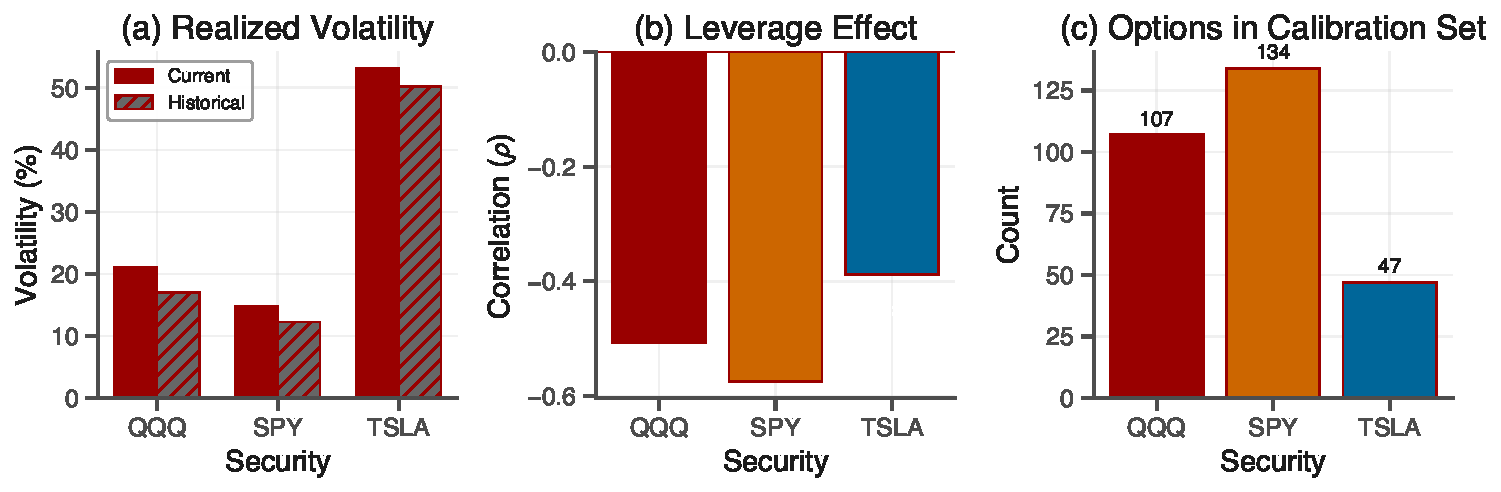
\includegraphics[width=0.85\textwidth]{figures/security_characteristics.pdf}
        \caption{Underlying security volatility and liquidity characteristics}
    \end{figure}
\end{frame}

%-------------------------------------------
% APPENDIX SECTION: Terminal Distributions
%-------------------------------------------
\begin{frame}
    \begin{center}
        \vspace{2cm}
        {\LARGE \textbf{Appendix D}}\\[0.5cm]
        {\Large Terminal Price Distributions}\\[1cm]
        \textit{Monte Carlo Simulation Analysis with Q-Q Plots}
    \end{center}
\end{frame}

\begin{frame}{Terminal Distribution Analysis - QQQ}
    \begin{figure}
        \centering
        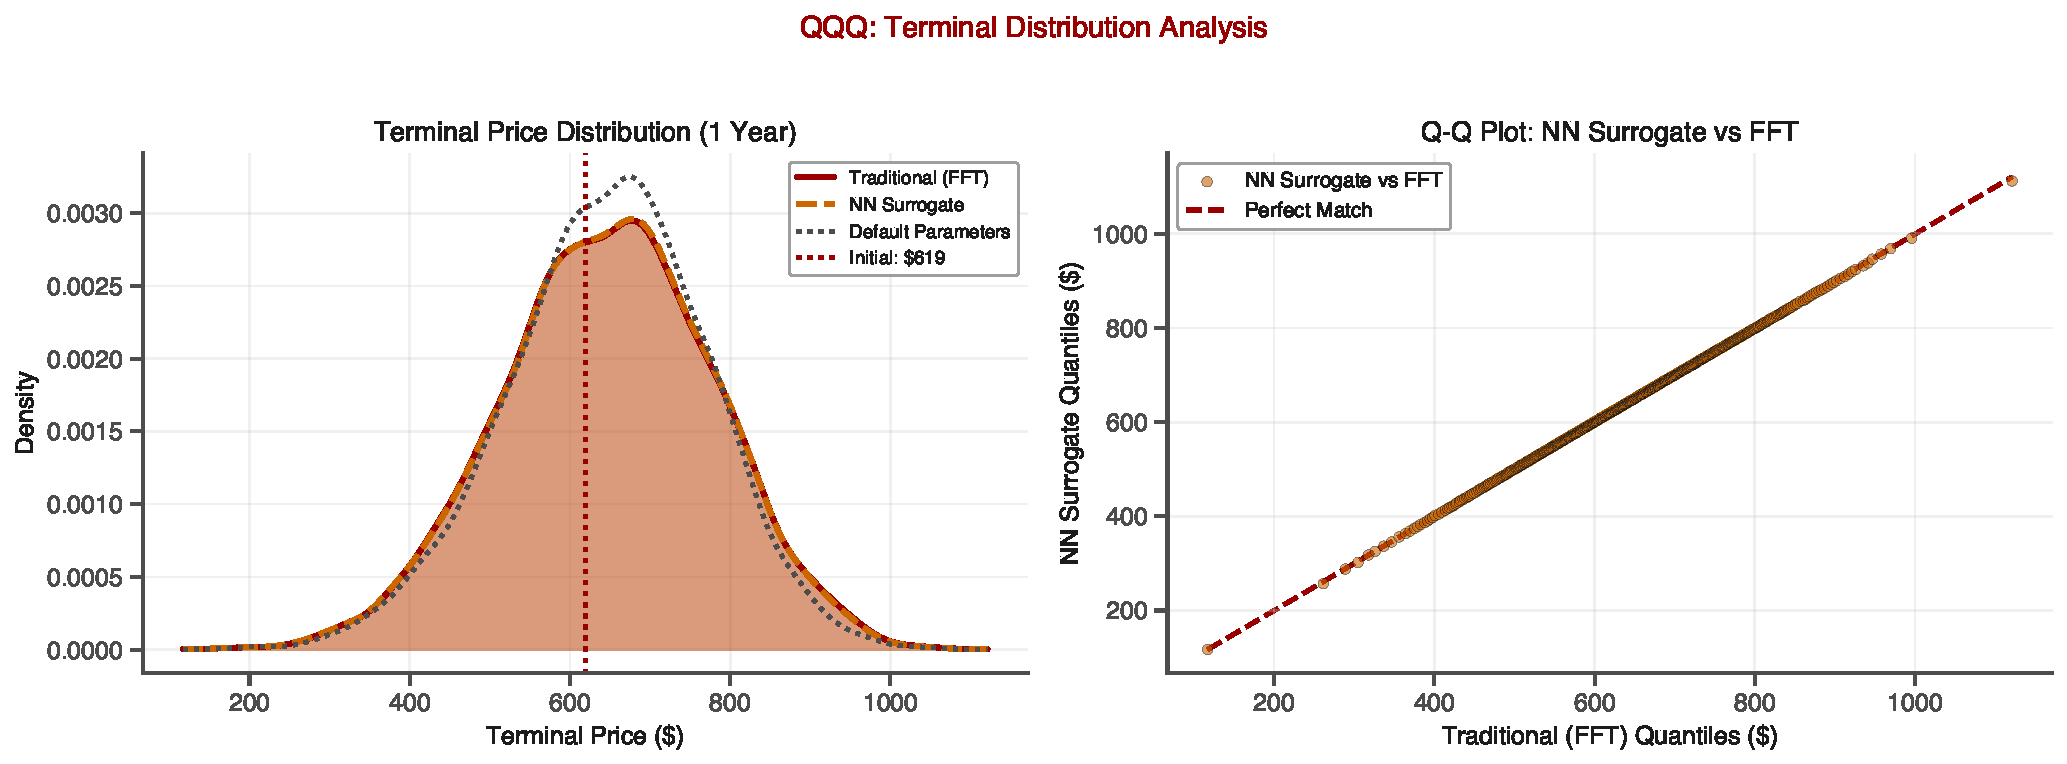
\includegraphics[width=0.95\textwidth]{figures/QQQ_terminal_dist_fft_vs_surrogate.pdf}
        \caption{QQQ: Terminal price distribution and Q-Q plot}
    \end{figure}
\end{frame}

\begin{frame}{Terminal Distribution Analysis - SPY}
    \begin{figure}
        \centering
        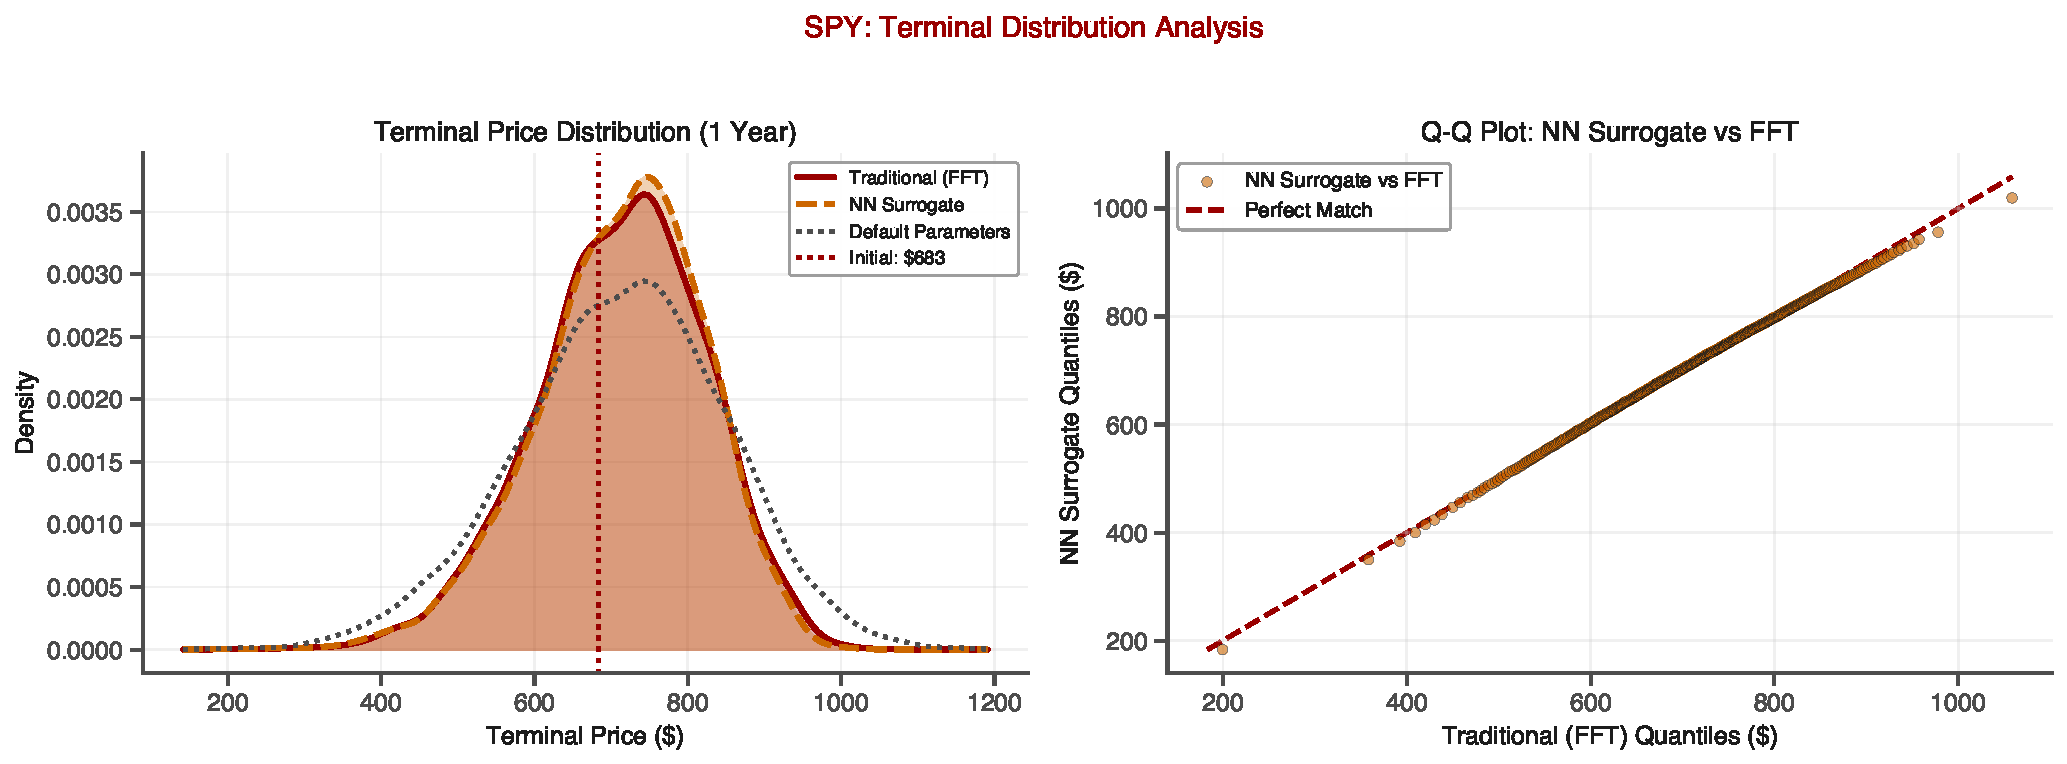
\includegraphics[width=0.95\textwidth]{figures/SPY_terminal_dist_fft_vs_surrogate.pdf}
        \caption{SPY: Terminal price distribution and Q-Q plot}
    \end{figure}
\end{frame}

\begin{frame}{Terminal Distribution Analysis - TSLA}
    \begin{figure}
        \centering
        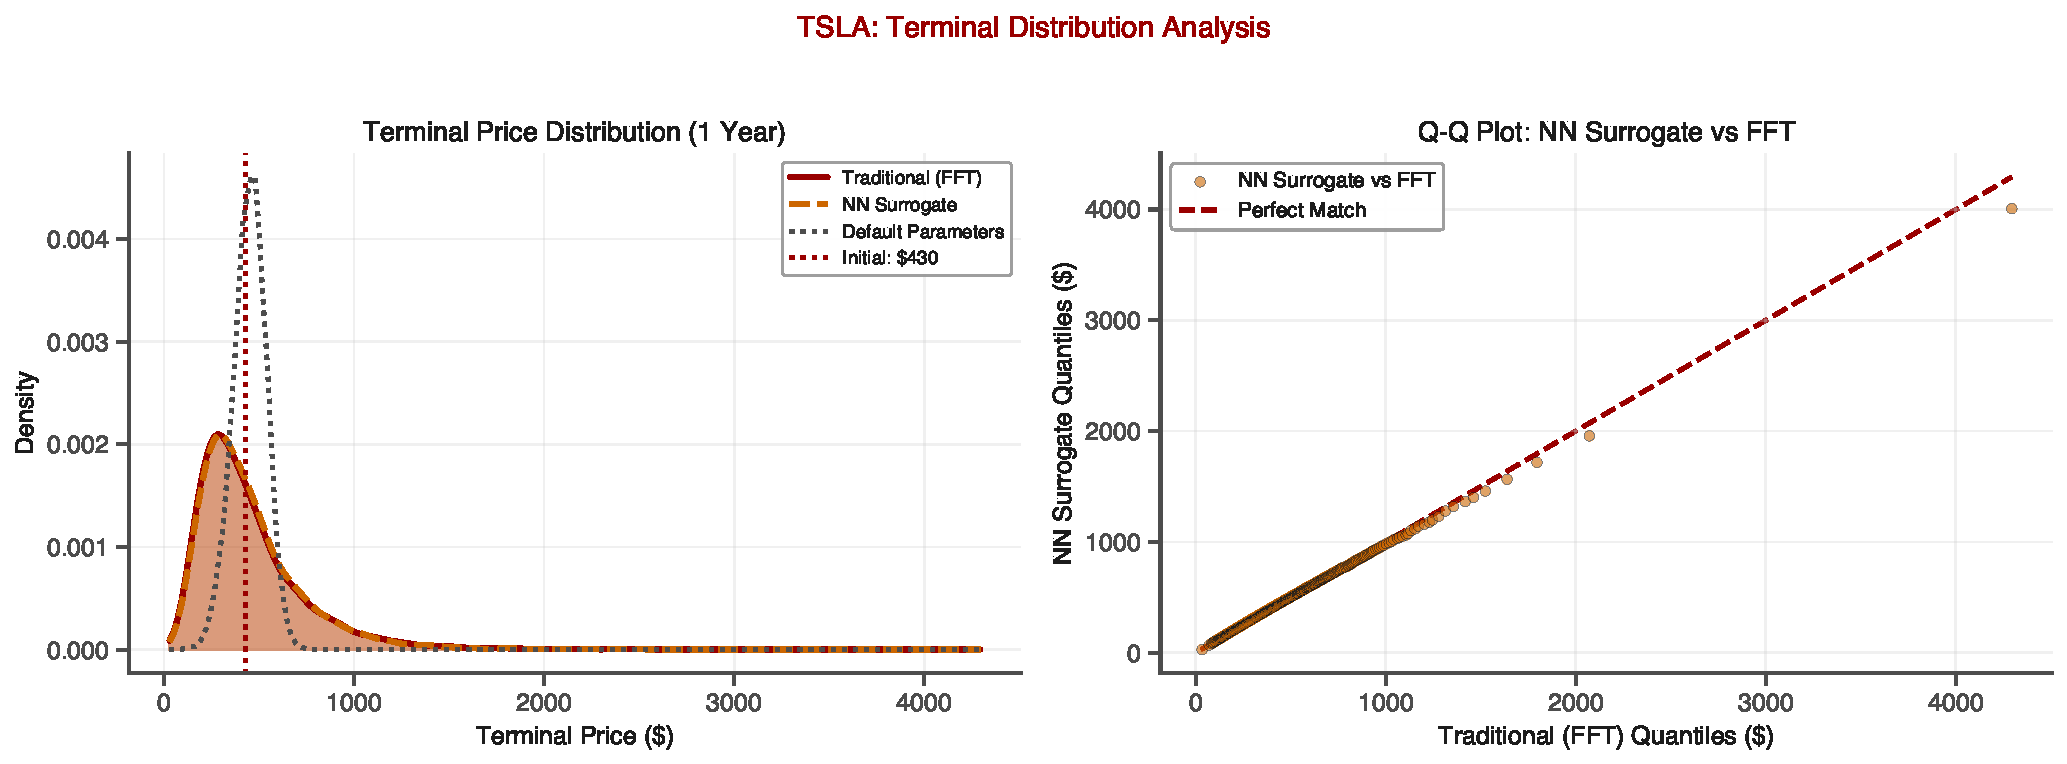
\includegraphics[width=0.95\textwidth]{figures/TSLA_terminal_dist_fft_vs_surrogate.pdf}
        \caption{TSLA: Terminal price distribution and Q-Q plot}
    \end{figure}
\end{frame}

%-------------------------------------------
% APPENDIX SECTION: Implied Volatility Surfaces
%-------------------------------------------
\begin{frame}
    \begin{center}
        \vspace{2cm}
        {\LARGE \textbf{Appendix E}}\\[0.5cm]
        {\Large Implied Volatility Surfaces}\\[1cm]
        \textit{Market vs Calibrated IV Surface Comparison}
    \end{center}
\end{frame}

\begin{frame}{QQQ IV Surface - Traditional vs Market}
    \begin{figure}
        \centering
        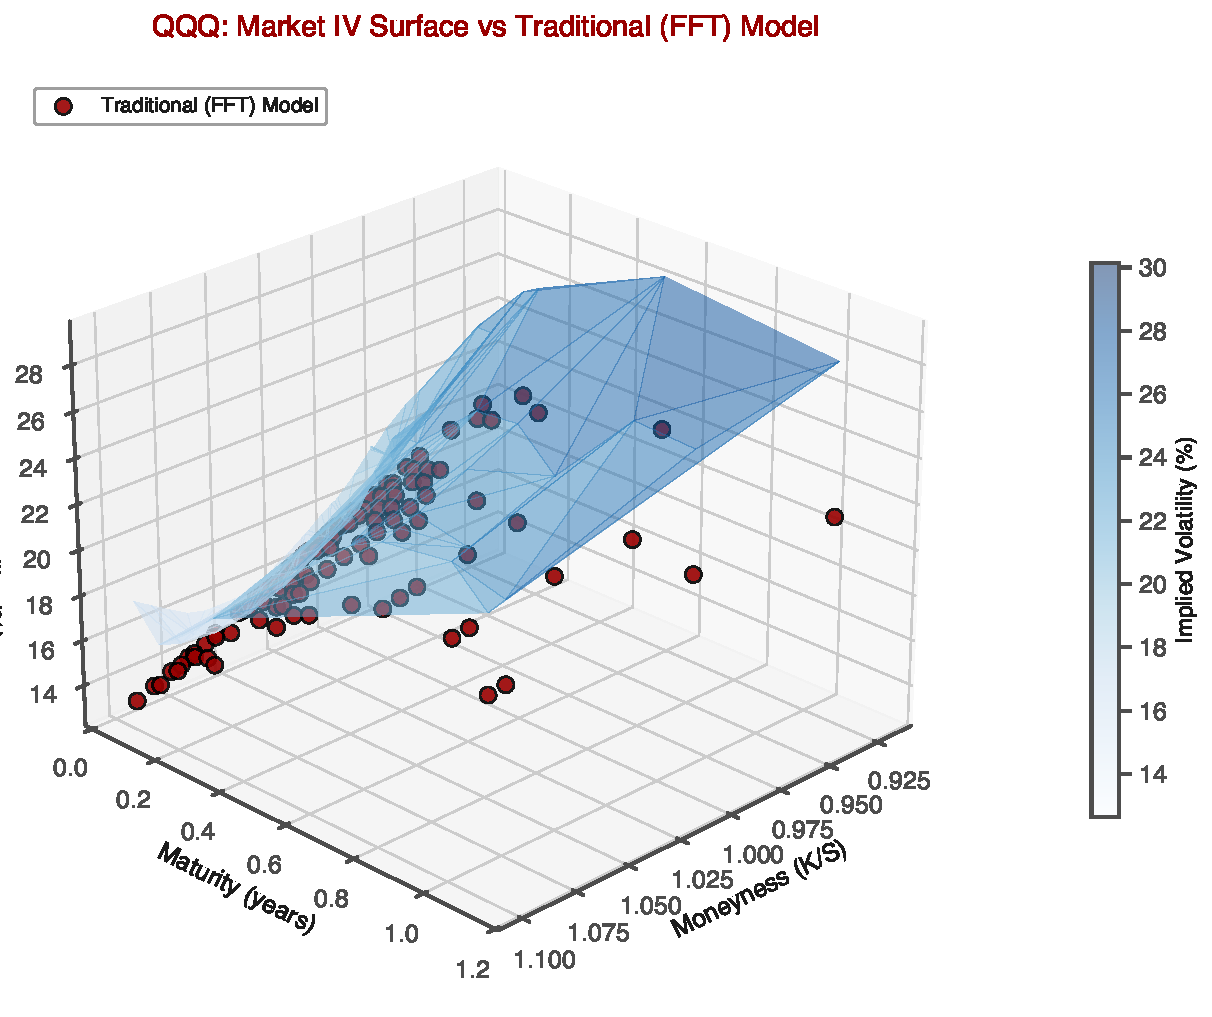
\includegraphics[width=0.65\textwidth]{figures/QQQ_iv_surface_fft.pdf}
        \caption{QQQ: Market IV surface vs Traditional (FFT) calibrated surface}
    \end{figure}
\end{frame}

\begin{frame}{QQQ IV Surface - NN vs Market}
    \begin{figure}
        \centering
        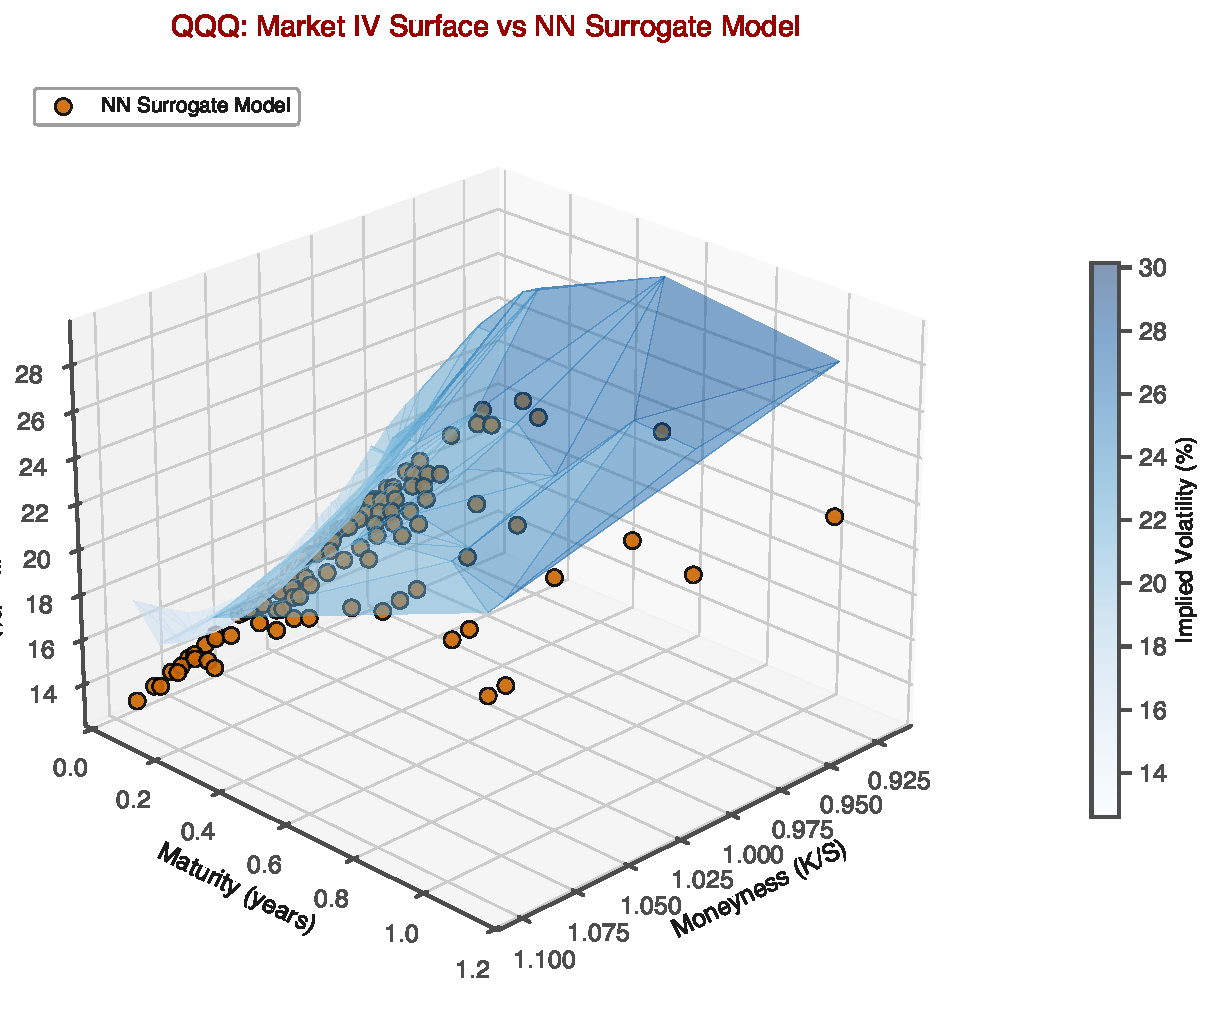
\includegraphics[width=0.65\textwidth]{figures/QQQ_iv_surface_nn.pdf}
        \caption{QQQ: Market IV surface vs NN Surrogate calibrated surface}
    \end{figure}
\end{frame}

\begin{frame}{SPY IV Surface - Traditional vs Market}
    \begin{figure}
        \centering
        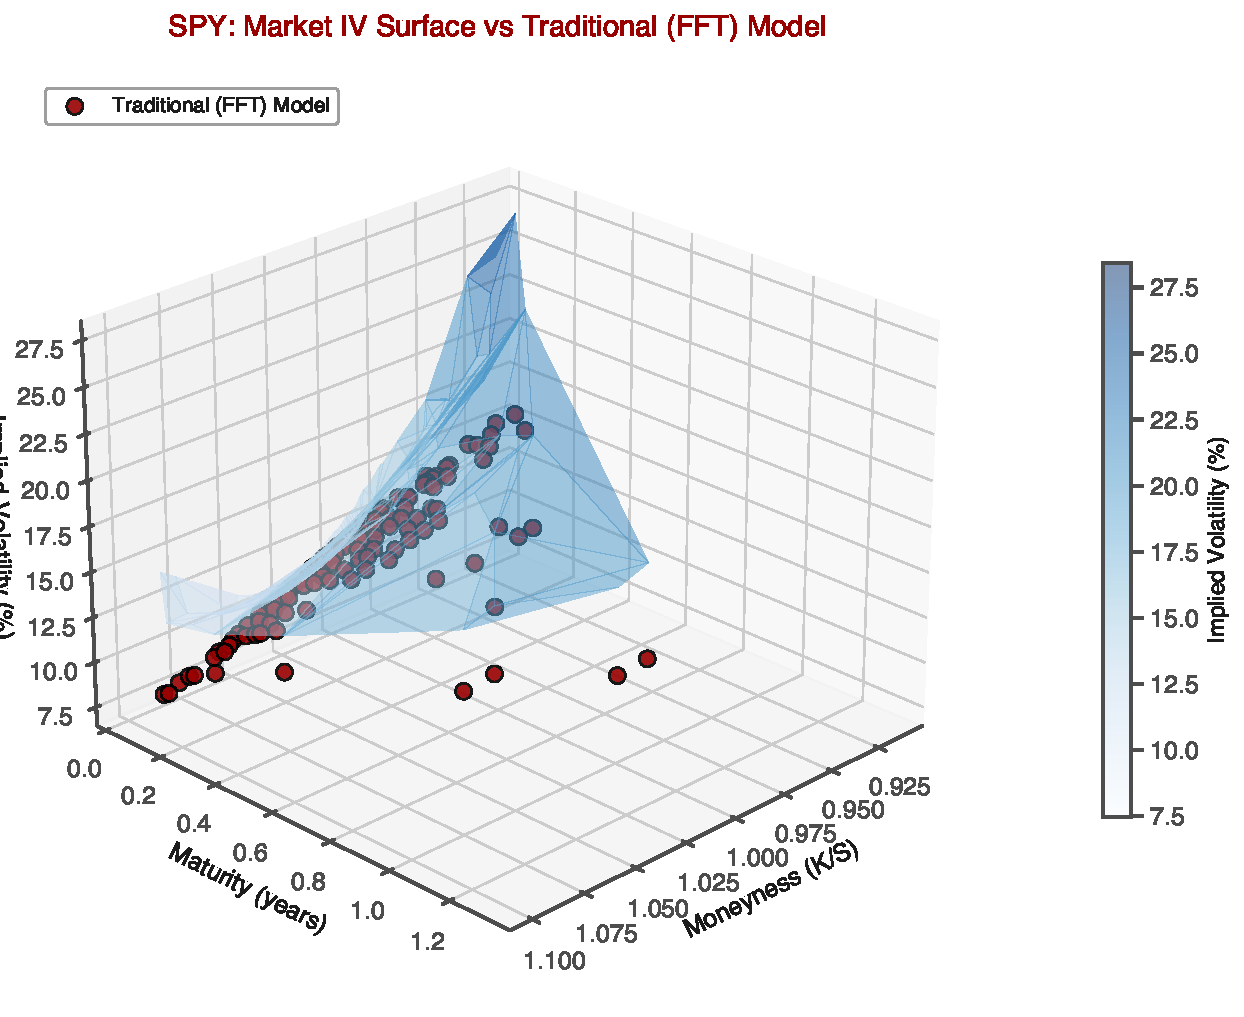
\includegraphics[width=0.65\textwidth]{figures/SPY_iv_surface_fft.pdf}
        \caption{SPY: Market IV surface vs Traditional (FFT) calibrated surface}
    \end{figure}
\end{frame}

\begin{frame}{SPY IV Surface - NN vs Market}
    \begin{figure}
        \centering
        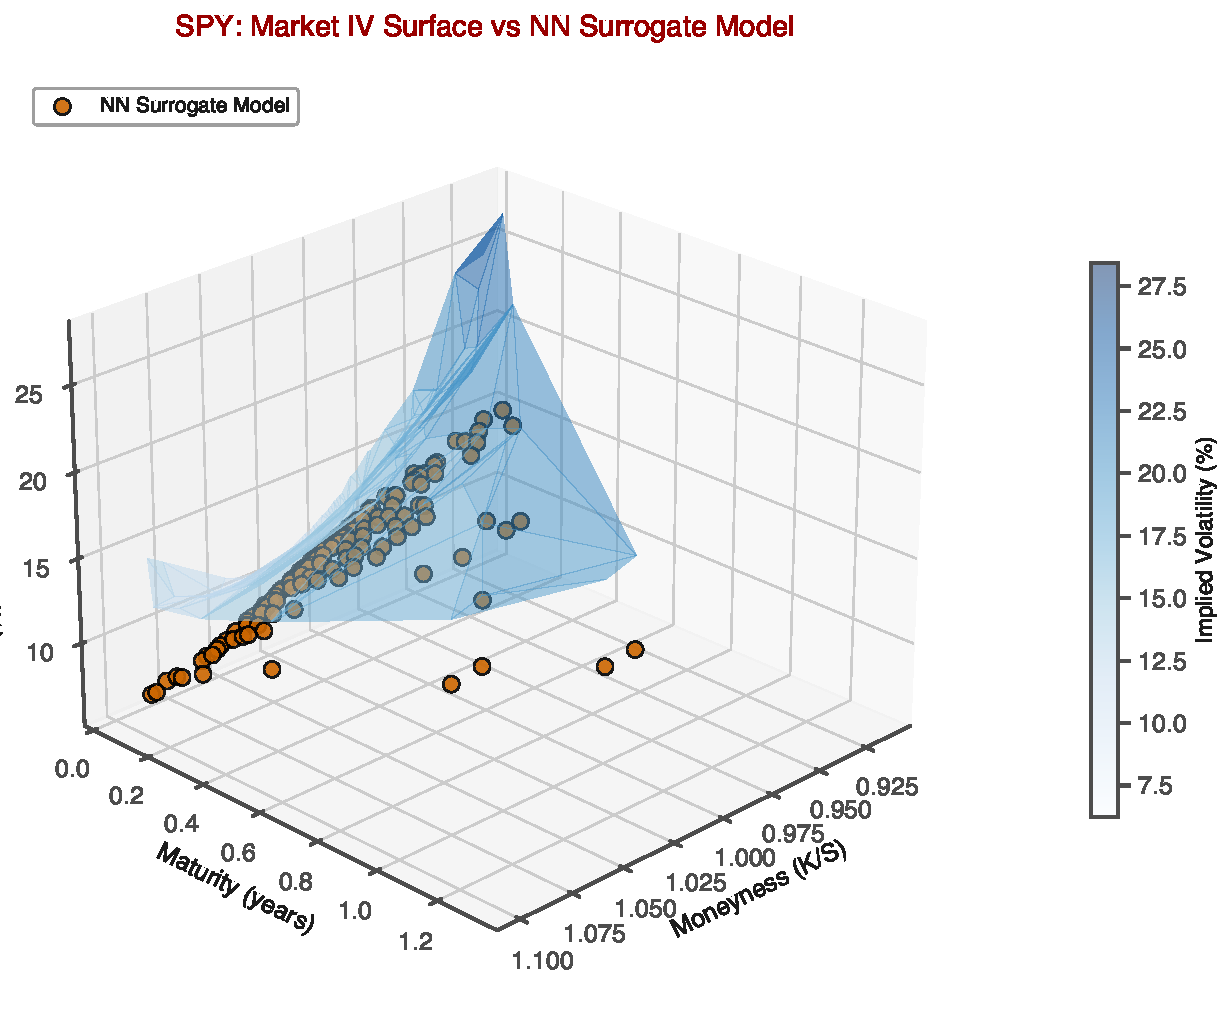
\includegraphics[width=0.65\textwidth]{figures/SPY_iv_surface_nn.pdf}
        \caption{SPY: Market IV surface vs NN Surrogate calibrated surface}
    \end{figure}
\end{frame}

\begin{frame}{TSLA IV Surface - Traditional vs Market}
    \begin{figure}
        \centering
        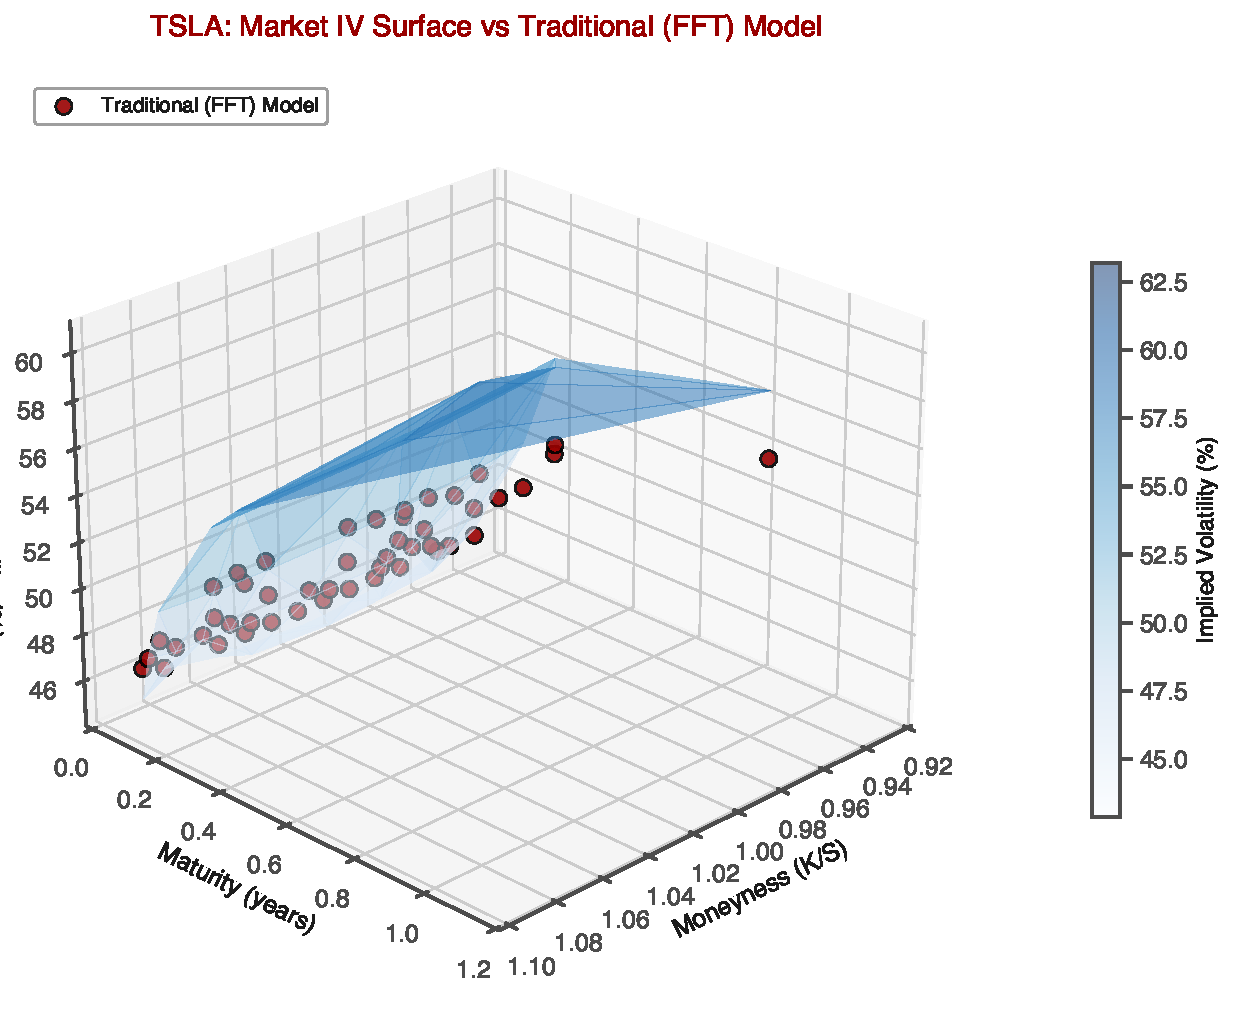
\includegraphics[width=0.65\textwidth]{figures/TSLA_iv_surface_fft.pdf}
        \caption{TSLA: Market IV surface vs Traditional (FFT) calibrated surface}
    \end{figure}
\end{frame}

\begin{frame}{TSLA IV Surface - NN vs Market}
    \begin{figure}
        \centering
        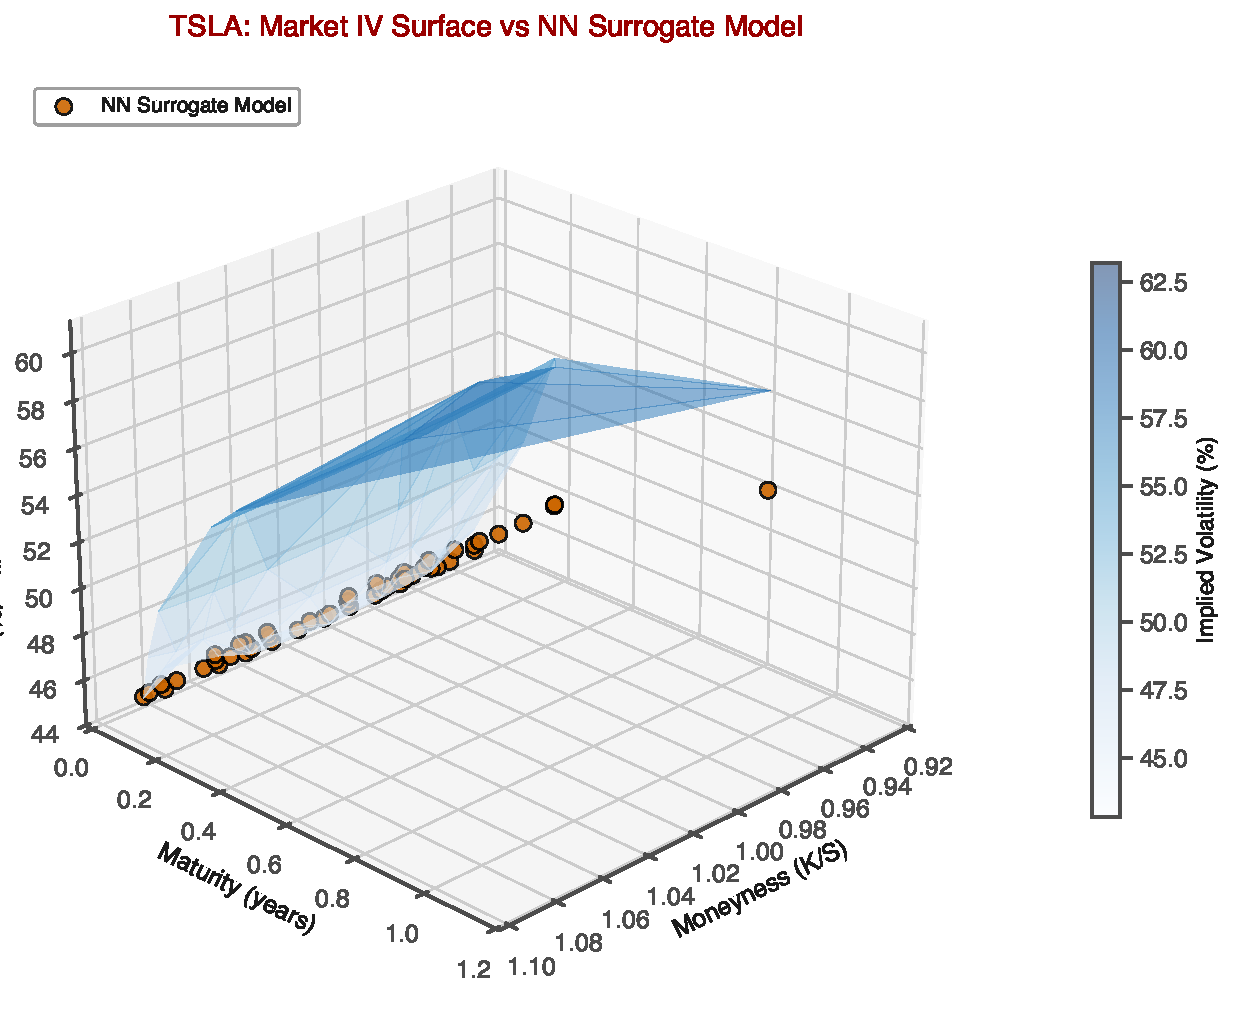
\includegraphics[width=0.65\textwidth]{figures/TSLA_iv_surface_nn.pdf}
        \caption{TSLA: Market IV surface vs NN Surrogate calibrated surface}
    \end{figure}
\end{frame}

%-------------------------------------------
% APPENDIX SECTION: Price Comparison Examples
%-------------------------------------------
\begin{frame}
    \begin{center}
        \vspace{2cm}
        {\LARGE \textbf{Appendix F}}\\[0.5cm]
        {\Large Price Comparison Examples}\\[1cm]
        \textit{NN vs FFT Price Predictions and Market Validation}
    \end{center}
\end{frame}

\begin{frame}{NN vs FFT: Price Prediction Comparison - Concrete Examples}
    \begin{figure}
        \centering
        \IfFileExists{figures/nn_vs_fft_examples.pdf}{%
            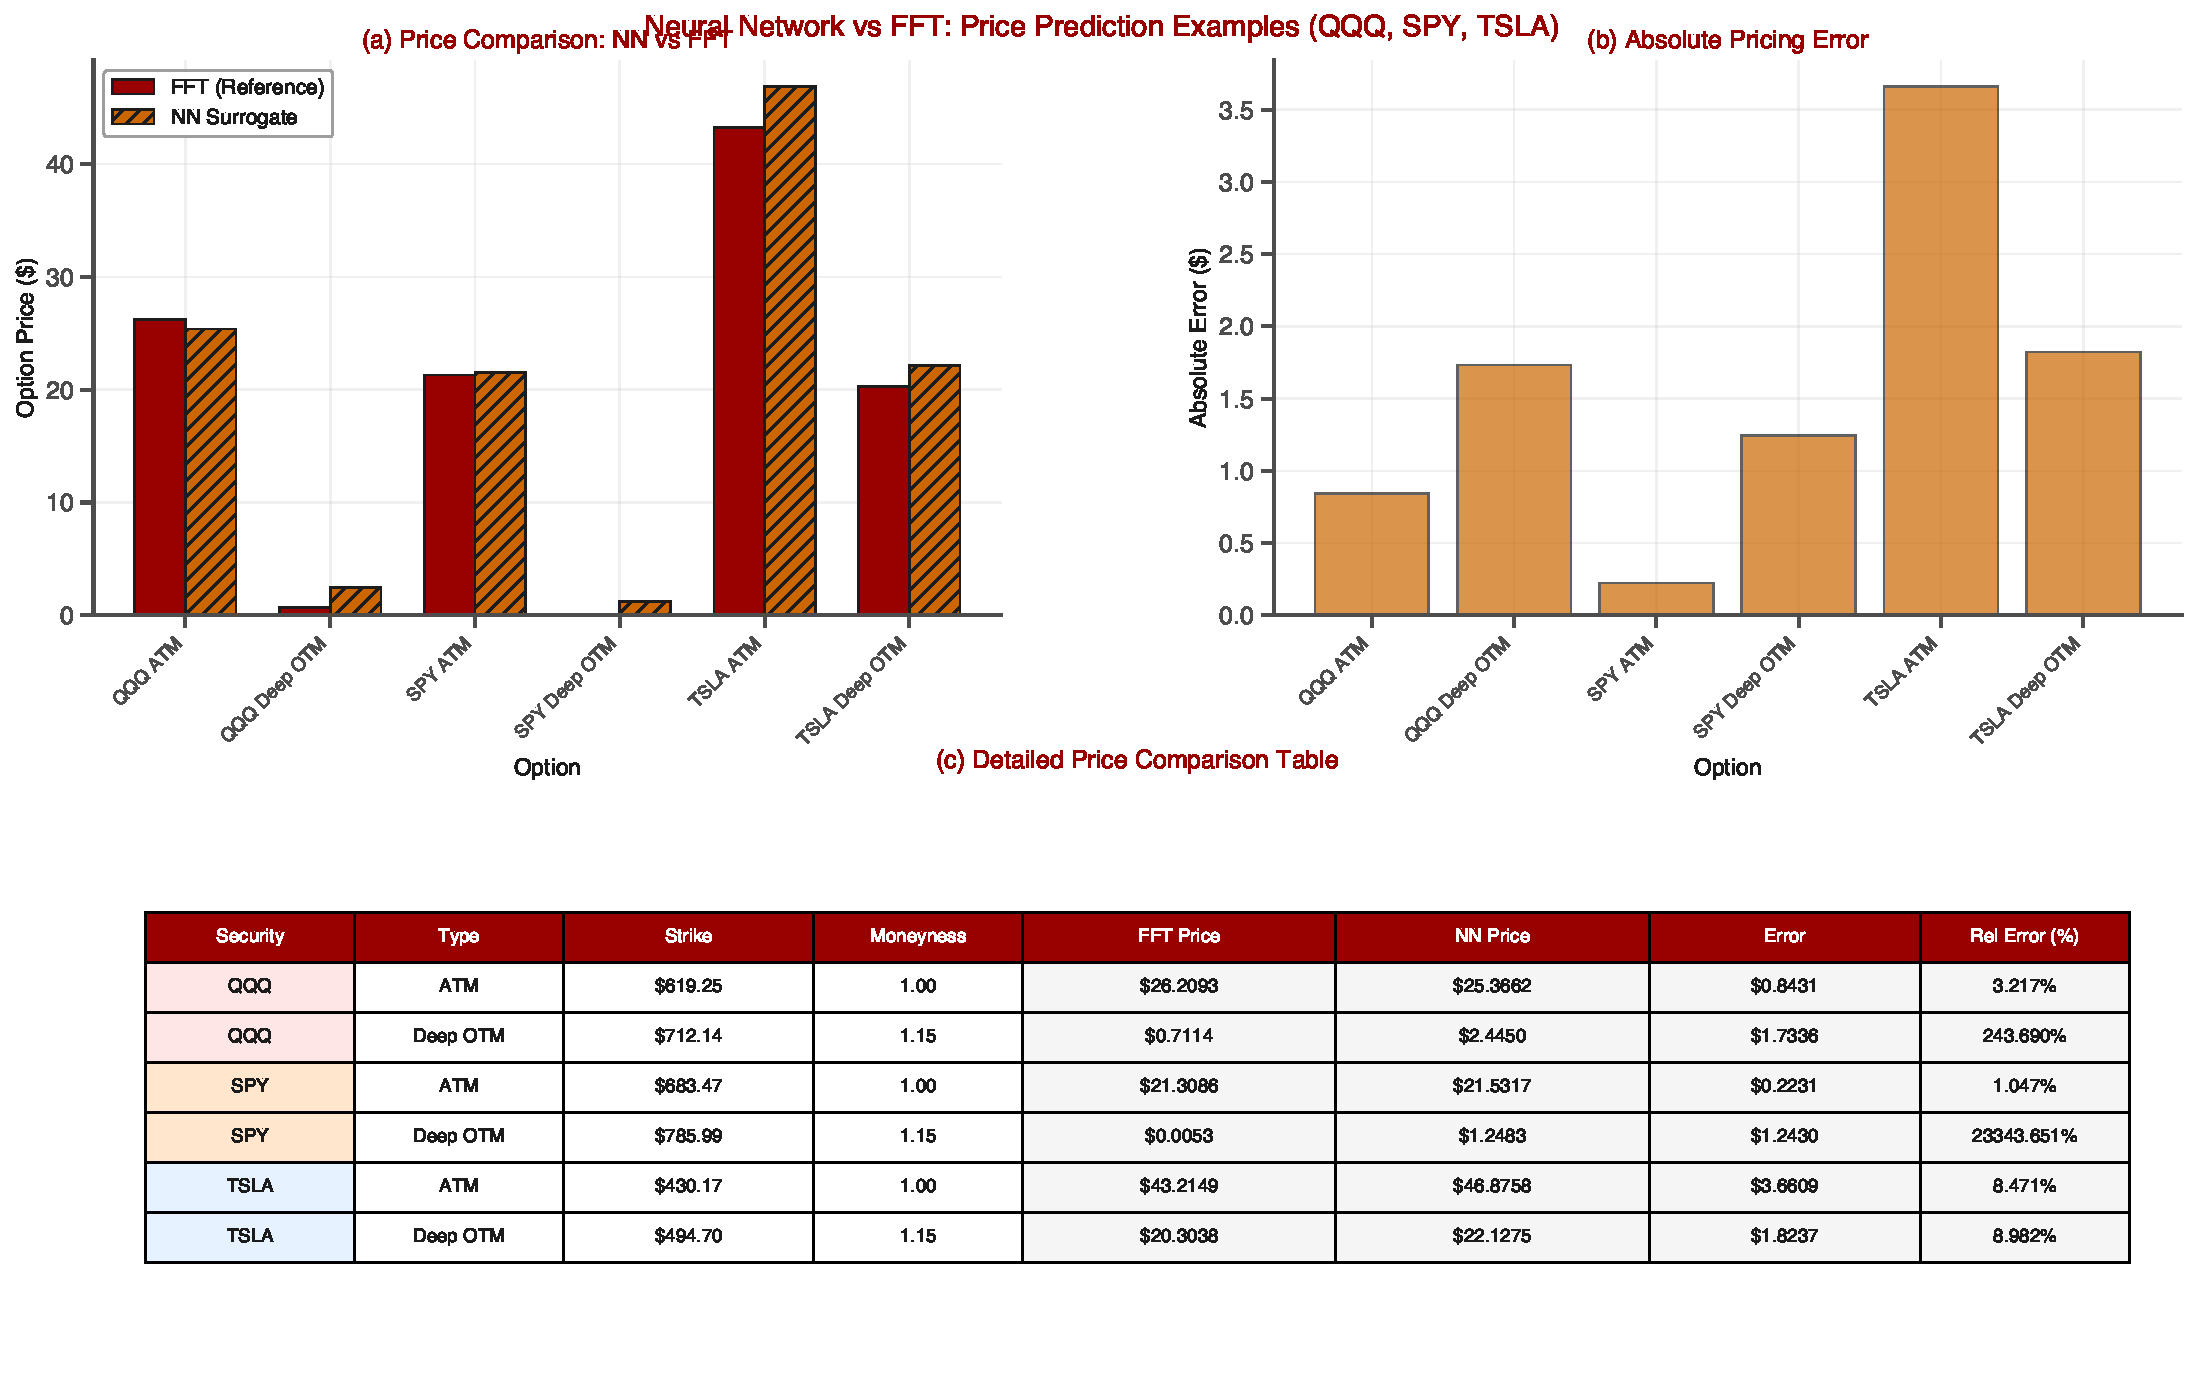
\includegraphics[width=0.95\textwidth]{figures/nn_vs_fft_examples.pdf}%
        }{%
            \fbox{\parbox{0.8\textwidth}{\centering
                \textbf{Figure will be generated}\\
                Execute the notebook cell in \texttt{presentation\_figures.ipynb}
            }}%
        }
        \caption{Comparison of NN surrogate and FFT pricing methods for different strikes and maturities}
    \end{figure}
\end{frame}

\begin{frame}{Market Price Validation}
    \begin{block}{Out-of-Sample Validation}
        Comparing calibrated model prices with current market prices from yfinance for ATM and OTM options.
    \end{block}
    
    \begin{figure}
        \centering
        \IfFileExists{figures/market_price_comparison.pdf}{%
            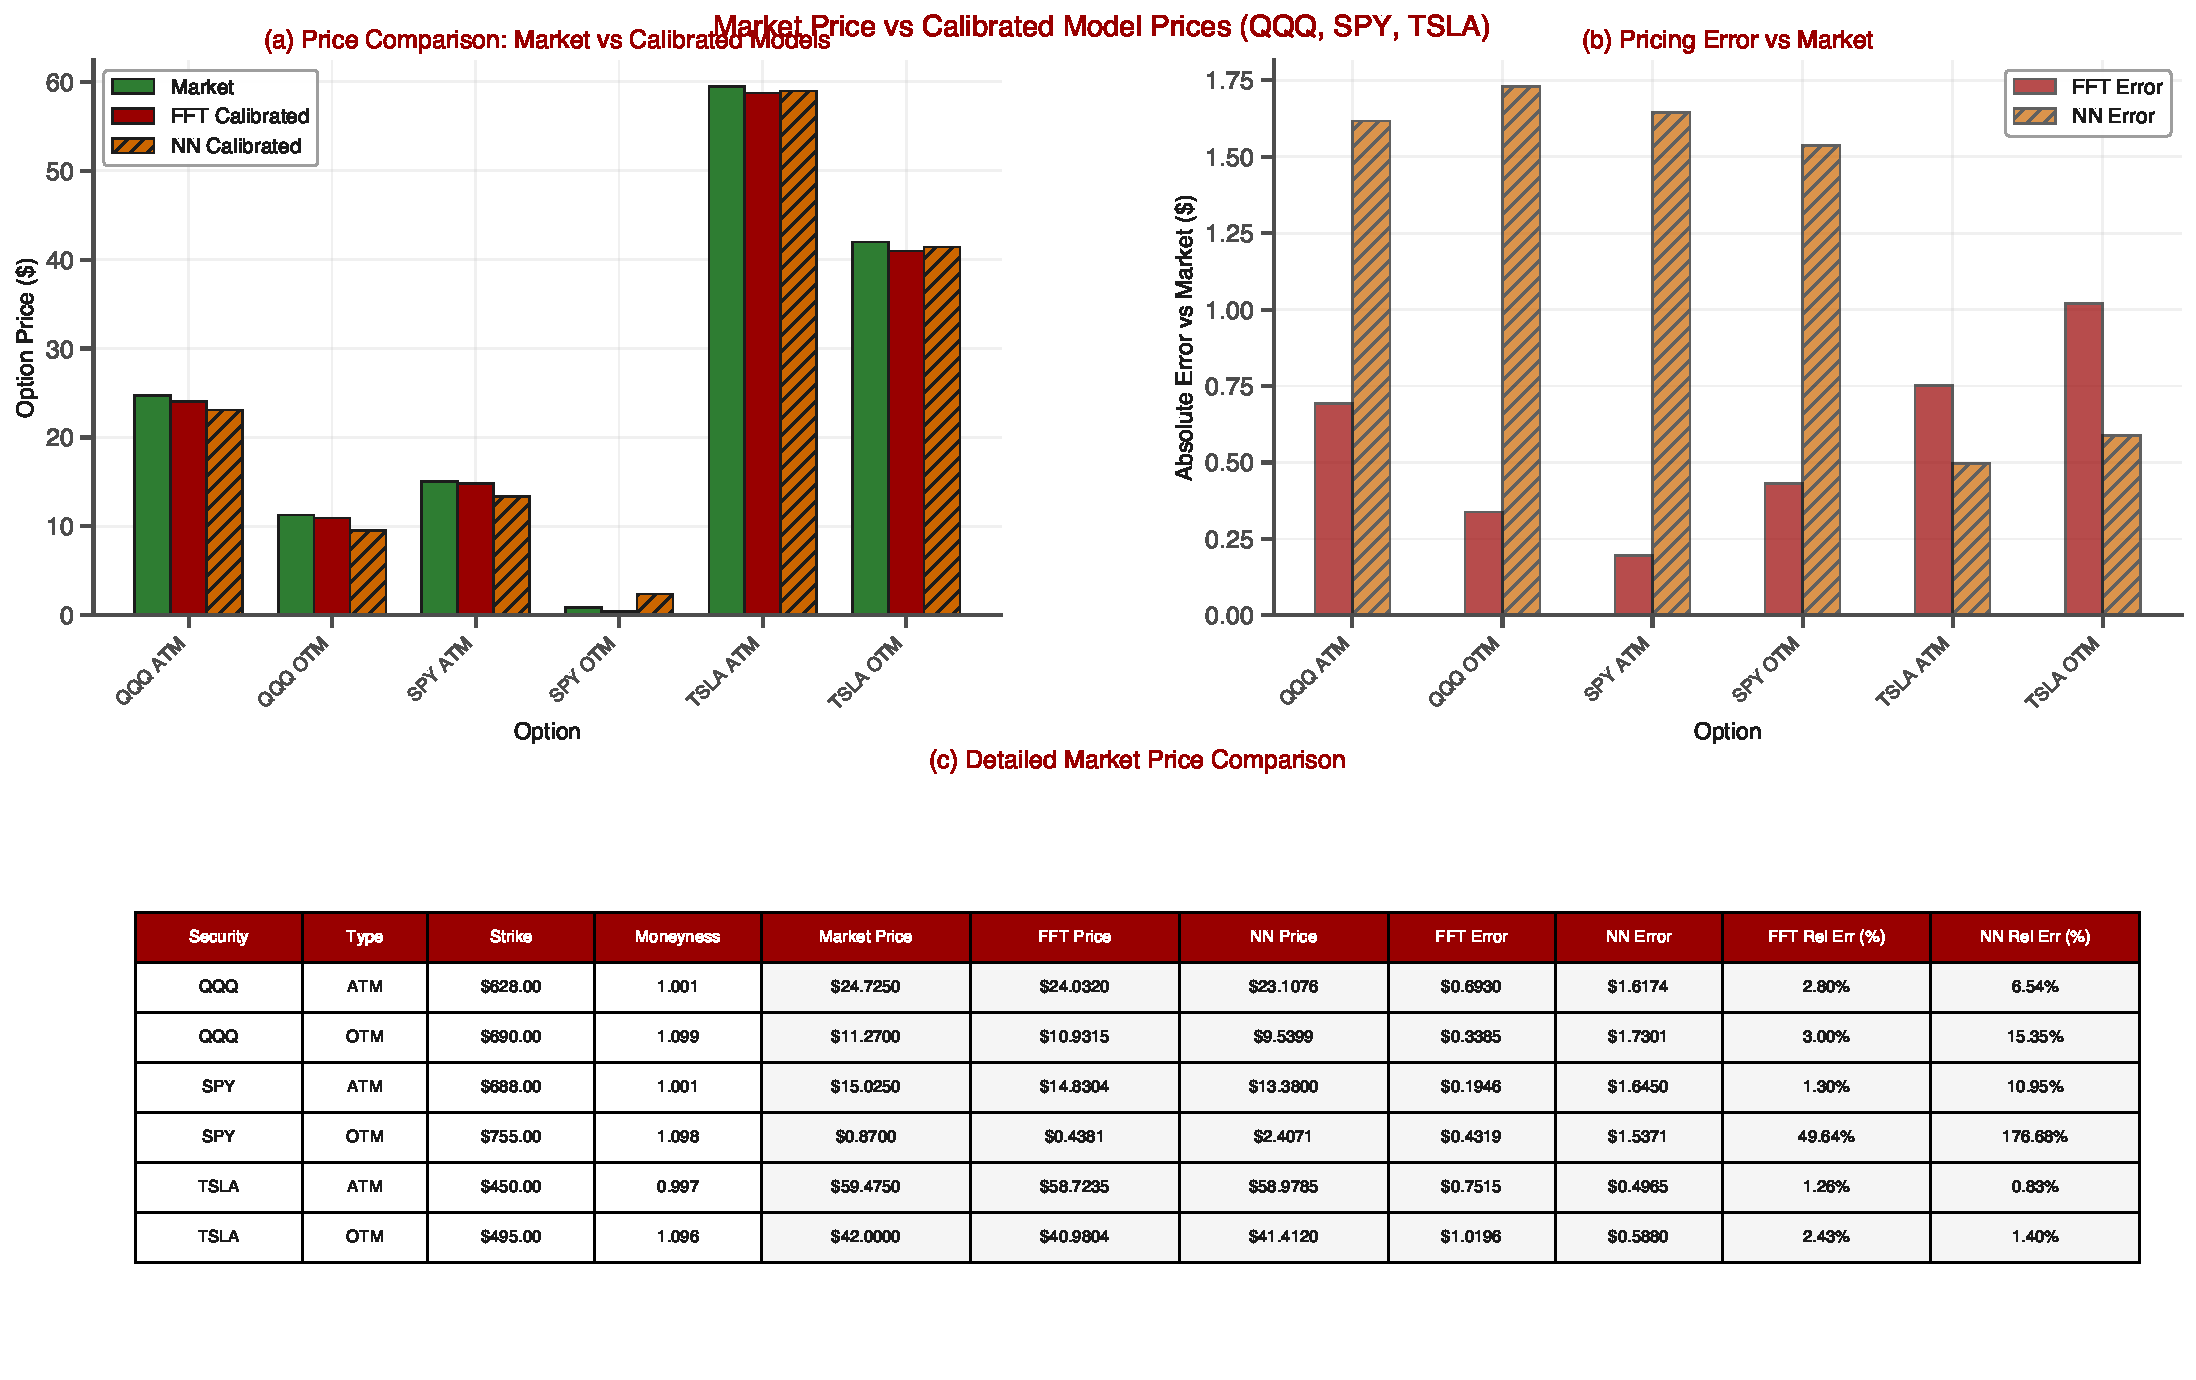
\includegraphics[width=0.95\textwidth]{figures/market_price_comparison.pdf}%
        }{%
            \fbox{\parbox{0.8\textwidth}{\centering
                \textbf{Figure will be generated}\\
                Execute the notebook cell in \texttt{presentation\_figures.ipynb}
            }}%
        }
        \caption{Market prices vs calibrated model prices (FFT and NN) for QQQ, SPY, TSLA}
    \end{figure}
    
    \footnotesize
    \begin{itemize}
        \item \textbf{Market data:} Current option prices from yfinance
        \item \textbf{Models:} Pre-calibrated parameters (no recalibration)
        \item \textbf{Insight:} Shows how well calibrated models match current market pricing
    \end{itemize}
\end{frame}

%-------------------------------------------
% APPENDIX SECTION: Pricing Methods Benchmark
%-------------------------------------------
\begin{frame}
    \begin{center}
        \vspace{2cm}
        {\LARGE \textbf{Appendix G}}\\[0.5cm]
        {\Large Pricing Methods Performance Benchmark}\\[1cm]
        \textit{Non-Calibrated Methods: Accuracy vs Speed Comparison}
    \end{center}
\end{frame}

\begin{frame}{Pricing Methods Performance Benchmark}
    \begin{figure}
        \centering
        \IfFileExists{figures/pricing_methods_benchmark.pdf}{%
            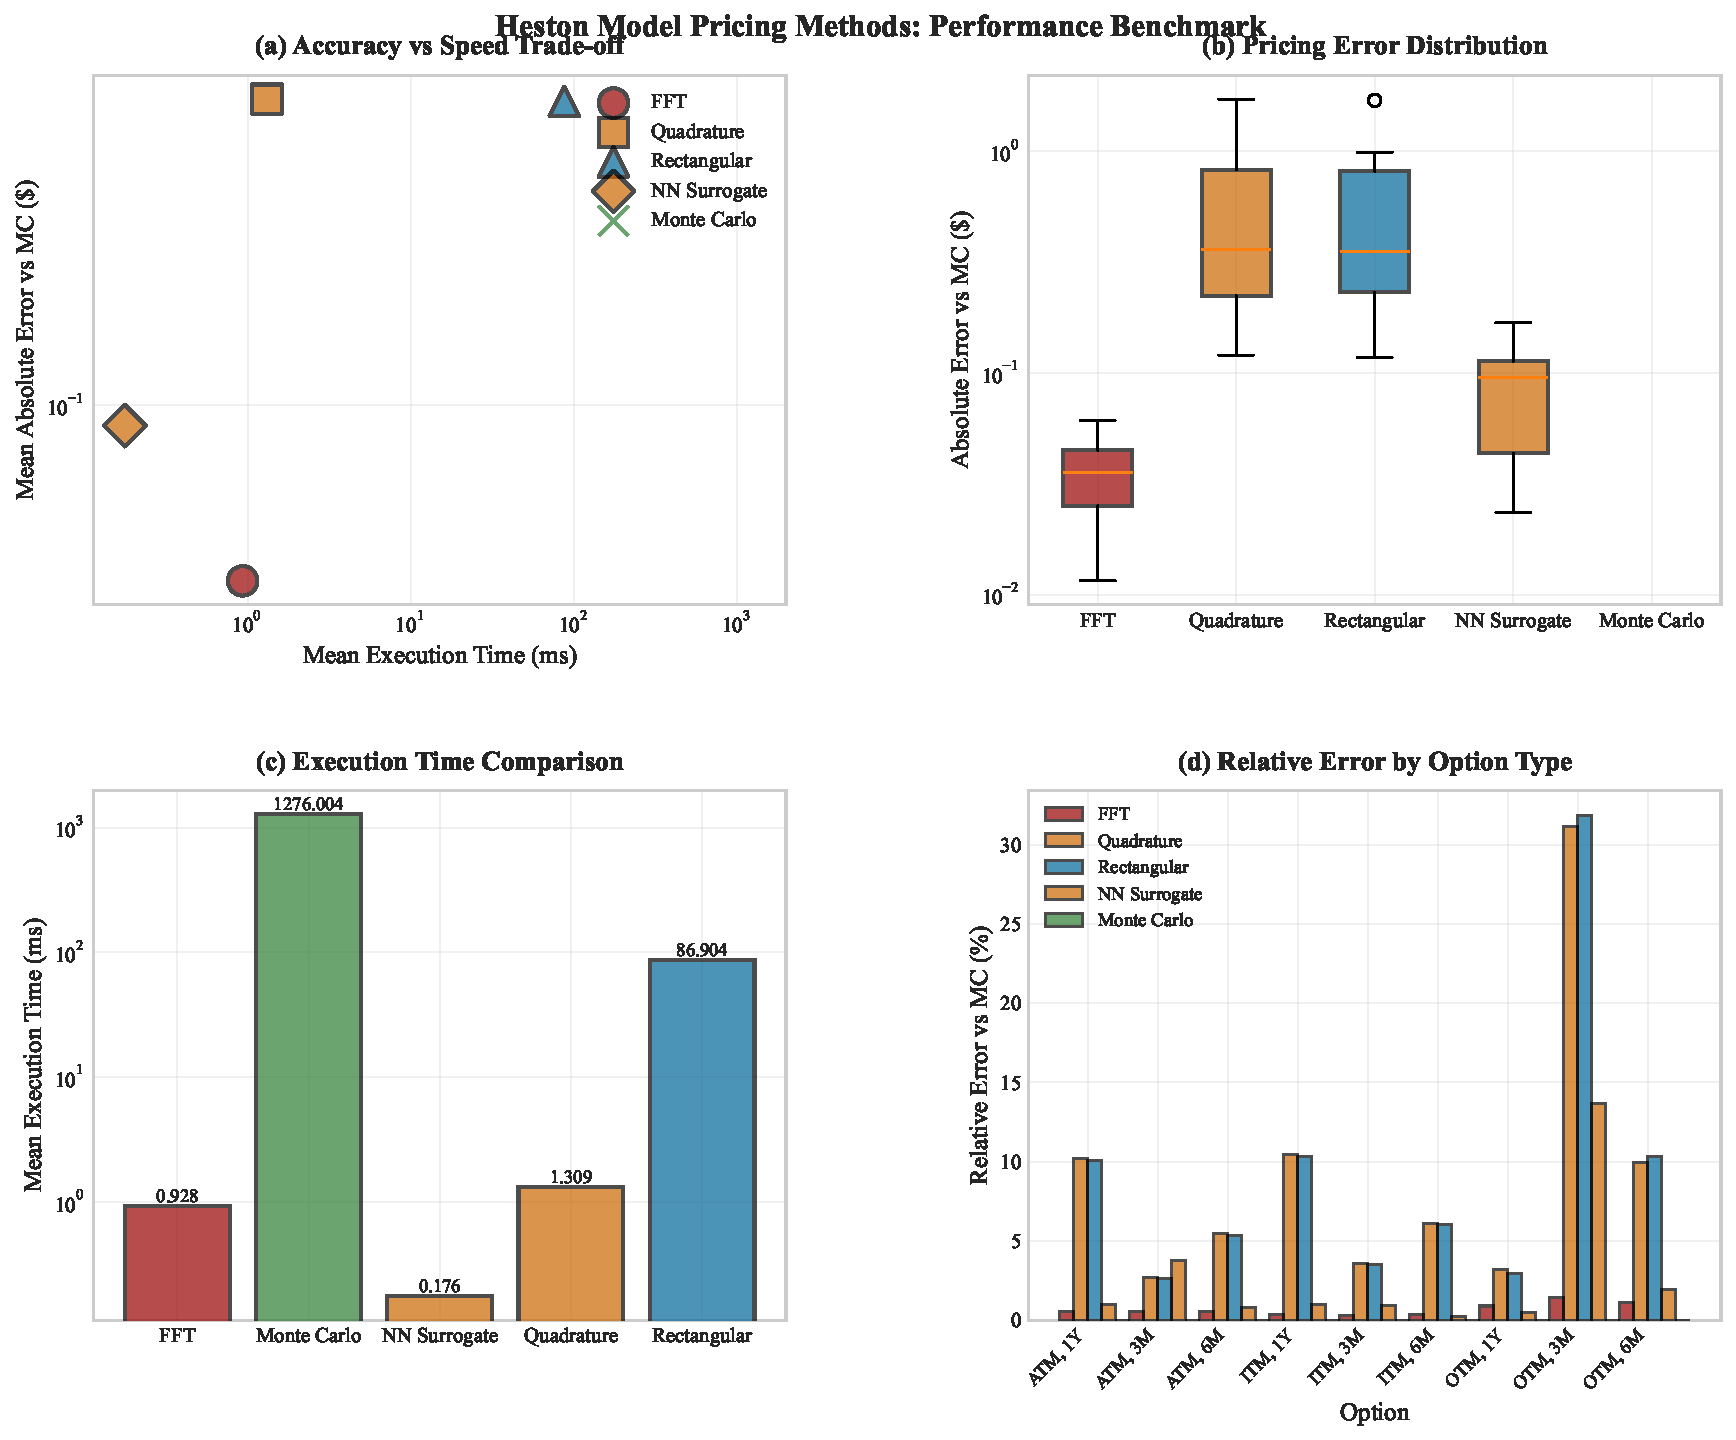
\includegraphics[width=0.80\textwidth]{figures/pricing_methods_benchmark.pdf}%
        }{%
            \fbox{\parbox{0.7\textwidth}{\centering
                \textbf{Figure will be generated}\\
                Execute section 6 in \texttt{heston\_model\_pricing.ipynb}
            }}%
        }
        \caption{Performance comparison: (a) Accuracy vs Speed trade-off, (b) Error distribution, (c) Execution time, (d) Relative error by option type}
    \end{figure}
\end{frame}

%-------------------------------------------
% APPENDIX SECTION: Exotic Options
%-------------------------------------------
\begin{frame}
    \begin{center}
        \vspace{2cm}
        {\LARGE \textbf{Appendix H}}\\[0.5cm]
        {\Large Exotic Options Pricing}\\[1cm]
        \textit{Monte Carlo Simulation with Calibrated Parameters}
    \end{center}
\end{frame}

\begin{frame}{Exotic Options Pricing}
    \begin{block}{Monte Carlo Simulation with Calibrated Parameters}
        Using calibrated Heston parameters from each method to price path-dependent exotics:
    \end{block}

    \vspace{0.2cm}

    \begin{columns}
        \begin{column}{0.5\textwidth}
            \textbf{Digital (Binary) Option:}
            \begin{itemize}
                \item Pays \$1 if $S_T > K$
                \item European-style payoff
                \item 100,000 MC paths
            \end{itemize}
            \begin{equation}
                V = e^{-rT} \mathbb{E}[\mathbf{1}_{S_T > K}]
            \end{equation}
        \end{column}
        \begin{column}{0.5\textwidth}
            \textbf{One-Touch Up Option:}
            \begin{itemize}
                \item Pays \$1 when $S_t \geq B$
                \item Path-dependent barrier
                \item Early termination
            \end{itemize}
            \begin{equation}
                V = e^{-r\tau} \mathbb{E}[\mathbf{1}_{\tau \leq T}]
            \end{equation}
        \end{column}
    \end{columns}
\end{frame}

\begin{frame}{Exotic Options Results}
    \begin{block}{Pricing Comparison (QQQ, $T=0.5$y, Barrier/Strike = 110\% of spot)}
    \end{block}

    \vspace{0.1cm}

    \begin{table}
        \centering
        \begin{tabular}{lccc}
            \toprule
            \textbf{Option Type} & \textbf{Classic FFT} & \textbf{NN Surrogate} & \textbf{Difference} \\
            \midrule
            Digital Call & \$0.364 $\pm$ 0.001 & \$0.339 $\pm$ 0.001 & $-6.8\%$ \\
            One-Touch Up & \$0.594 $\pm$ 0.002 & \$0.716 $\pm$ 0.001 & $+20.5\%$ \\
            \bottomrule
        \end{tabular}
    \end{table}

    \vspace{0.2cm}

    \begin{alertblock}{Key Insight}
        Path-dependent options (One-Touch) show larger pricing differences due to sensitivity to volatility dynamics. Digital options (terminal payoff only) show smaller differences.
    \end{alertblock}

    \vspace{0.1cm}

    \small
    \textit{Results from Monte Carlo simulation with 100,000 paths per option.}
\end{frame}

\end{document}
